\documentclass[a4paper]{book}
\usepackage{makeidx}
\usepackage{natbib}
\usepackage{graphicx}
\usepackage{multicol}
\usepackage{float}
\usepackage{listings}
\usepackage{color}
\usepackage{ifthen}
\usepackage[table]{xcolor}
\usepackage{textcomp}
\usepackage{alltt}
\usepackage{ifpdf}
\ifpdf
\usepackage[pdftex,
            pagebackref=true,
            colorlinks=true,
            linkcolor=blue,
            unicode
           ]{hyperref}
\else
\usepackage[ps2pdf,
            pagebackref=true,
            colorlinks=true,
            linkcolor=blue,
            unicode
           ]{hyperref}
\usepackage{pspicture}
\fi
\usepackage[utf8]{inputenc}
\usepackage{mathptmx}
\usepackage[scaled=.90]{helvet}
\usepackage{courier}
\usepackage{sectsty}
\usepackage[titles]{tocloft}
\usepackage{doxygen}
\lstset{language=C++,inputencoding=utf8,basicstyle=\footnotesize,breaklines=true,breakatwhitespace=true,tabsize=8,numbers=left }
\makeindex
\setcounter{tocdepth}{3}
\renewcommand{\footrulewidth}{0.4pt}
\renewcommand{\familydefault}{\sfdefault}
\hfuzz=15pt
\setlength{\emergencystretch}{15pt}
\hbadness=750
\tolerance=750
\begin{document}
\hypersetup{pageanchor=false,citecolor=blue}
\begin{titlepage}
\vspace*{7cm}
\begin{center}
{\Large \-My \-Project }\\
\vspace*{1cm}
{\large \-Generated by Doxygen 1.7.6.1}\\
\vspace*{0.5cm}
{\small Sun Jun 16 2013 21:28:48}\\
\end{center}
\end{titlepage}
\clearemptydoublepage
\pagenumbering{roman}
\tableofcontents
\clearemptydoublepage
\pagenumbering{arabic}
\hypersetup{pageanchor=true,citecolor=blue}
\chapter{\-Class \-Index}
\section{\-Class \-Hierarchy}
\-This inheritance list is sorted roughly, but not completely, alphabetically\-:\begin{DoxyCompactList}
\item \contentsline{section}{\-Config}{\pageref{classConfig}}{}
\item \contentsline{section}{\-Config\-Manager}{\pageref{classConfigManager}}{}
\item \contentsline{section}{\-Doc\-Button}{\pageref{classDocButton}}{}
\item \contentsline{section}{\-Main\-Window}{\pageref{classMainWindow}}{}
\item \contentsline{section}{\-Note}{\pageref{classNote}}{}
\begin{DoxyCompactList}
\item \contentsline{section}{\-Article}{\pageref{classArticle}}{}
\item \contentsline{section}{\-Binary}{\pageref{classBinary}}{}
\begin{DoxyCompactList}
\item \contentsline{section}{\-Audio}{\pageref{classAudio}}{}
\item \contentsline{section}{\-Image}{\pageref{classImage}}{}
\item \contentsline{section}{\-Video}{\pageref{classVideo}}{}
\end{DoxyCompactList}
\item \contentsline{section}{\-Document}{\pageref{classDocument}}{}
\end{DoxyCompactList}
\item \contentsline{section}{\-Note\-Editor}{\pageref{classNoteEditor}}{}
\begin{DoxyCompactList}
\item \contentsline{section}{\-Article\-Editor}{\pageref{classArticleEditor}}{}
\item \contentsline{section}{\-Binary\-Editor}{\pageref{classBinaryEditor}}{}
\begin{DoxyCompactList}
\item \contentsline{section}{\-Audio\-Editor}{\pageref{classAudioEditor}}{}
\item \contentsline{section}{\-Image\-Editor}{\pageref{classImageEditor}}{}
\item \contentsline{section}{\-Video\-Editor}{\pageref{classVideoEditor}}{}
\end{DoxyCompactList}
\item \contentsline{section}{\-Document\-Editor}{\pageref{classDocumentEditor}}{}
\end{DoxyCompactList}
\item \contentsline{section}{\-Notes\-Exception}{\pageref{classNotesException}}{}
\item \contentsline{section}{\-Notes\-Manager}{\pageref{classNotesManager}}{}
\item \contentsline{section}{\-Q\-List\-Editor}{\pageref{classQListEditor}}{}
\item \contentsline{section}{\-Q\-List\-Editor\-Item}{\pageref{classQListEditorItem}}{}
\item \contentsline{section}{\-Tag}{\pageref{classTag}}{}
\item \contentsline{section}{\-Tag\-Manager}{\pageref{classTagManager}}{}
\item \contentsline{section}{\-Workspace}{\pageref{classWorkspace}}{}
\end{DoxyCompactList}

\chapter{\-Class \-Index}
\section{\-Class \-List}
\-Here are the classes, structs, unions and interfaces with brief descriptions\-:\begin{DoxyCompactList}
\item\contentsline{section}{\hyperlink{classArticle}{\-Article} }{\pageref{classArticle}}{}
\item\contentsline{section}{\hyperlink{classArticleEditor}{\-Article\-Editor} }{\pageref{classArticleEditor}}{}
\item\contentsline{section}{\hyperlink{classAudio}{\-Audio} }{\pageref{classAudio}}{}
\item\contentsline{section}{\hyperlink{classAudioEditor}{\-Audio\-Editor} }{\pageref{classAudioEditor}}{}
\item\contentsline{section}{\hyperlink{classBinary}{\-Binary} }{\pageref{classBinary}}{}
\item\contentsline{section}{\hyperlink{classBinaryEditor}{\-Binary\-Editor} }{\pageref{classBinaryEditor}}{}
\item\contentsline{section}{\hyperlink{classConfig}{\-Config} }{\pageref{classConfig}}{}
\item\contentsline{section}{\hyperlink{classConfigManager}{\-Config\-Manager} }{\pageref{classConfigManager}}{}
\item\contentsline{section}{\hyperlink{classDocButton}{\-Doc\-Button} }{\pageref{classDocButton}}{}
\item\contentsline{section}{\hyperlink{classDocument}{\-Document} }{\pageref{classDocument}}{}
\item\contentsline{section}{\hyperlink{classDocumentEditor}{\-Document\-Editor} }{\pageref{classDocumentEditor}}{}
\item\contentsline{section}{\hyperlink{classImage}{\-Image} }{\pageref{classImage}}{}
\item\contentsline{section}{\hyperlink{classImageEditor}{\-Image\-Editor} }{\pageref{classImageEditor}}{}
\item\contentsline{section}{\hyperlink{classMainWindow}{\-Main\-Window} }{\pageref{classMainWindow}}{}
\item\contentsline{section}{\hyperlink{classNote}{\-Note} }{\pageref{classNote}}{}
\item\contentsline{section}{\hyperlink{classNoteEditor}{\-Note\-Editor} }{\pageref{classNoteEditor}}{}
\item\contentsline{section}{\hyperlink{classNotesException}{\-Notes\-Exception} }{\pageref{classNotesException}}{}
\item\contentsline{section}{\hyperlink{classNotesManager}{\-Notes\-Manager} }{\pageref{classNotesManager}}{}
\item\contentsline{section}{\hyperlink{classQListEditor}{\-Q\-List\-Editor} }{\pageref{classQListEditor}}{}
\item\contentsline{section}{\hyperlink{classQListEditorItem}{\-Q\-List\-Editor\-Item} }{\pageref{classQListEditorItem}}{}
\item\contentsline{section}{\hyperlink{classTag}{\-Tag} }{\pageref{classTag}}{}
\item\contentsline{section}{\hyperlink{classTagManager}{\-Tag\-Manager} }{\pageref{classTagManager}}{}
\item\contentsline{section}{\hyperlink{classVideo}{\-Video} }{\pageref{classVideo}}{}
\item\contentsline{section}{\hyperlink{classVideoEditor}{\-Video\-Editor} }{\pageref{classVideoEditor}}{}
\item\contentsline{section}{\hyperlink{classWorkspace}{\-Workspace} }{\pageref{classWorkspace}}{}
\end{DoxyCompactList}

\chapter{\-Class \-Documentation}
\hypertarget{classArticle}{\section{\-Article \-Class \-Reference}
\label{classArticle}\index{\-Article@{\-Article}}
}


{\ttfamily \#include $<$\-Article.\-h$>$}

\-Inheritance diagram for \-Article\-:\begin{figure}[H]
\begin{center}
\leavevmode
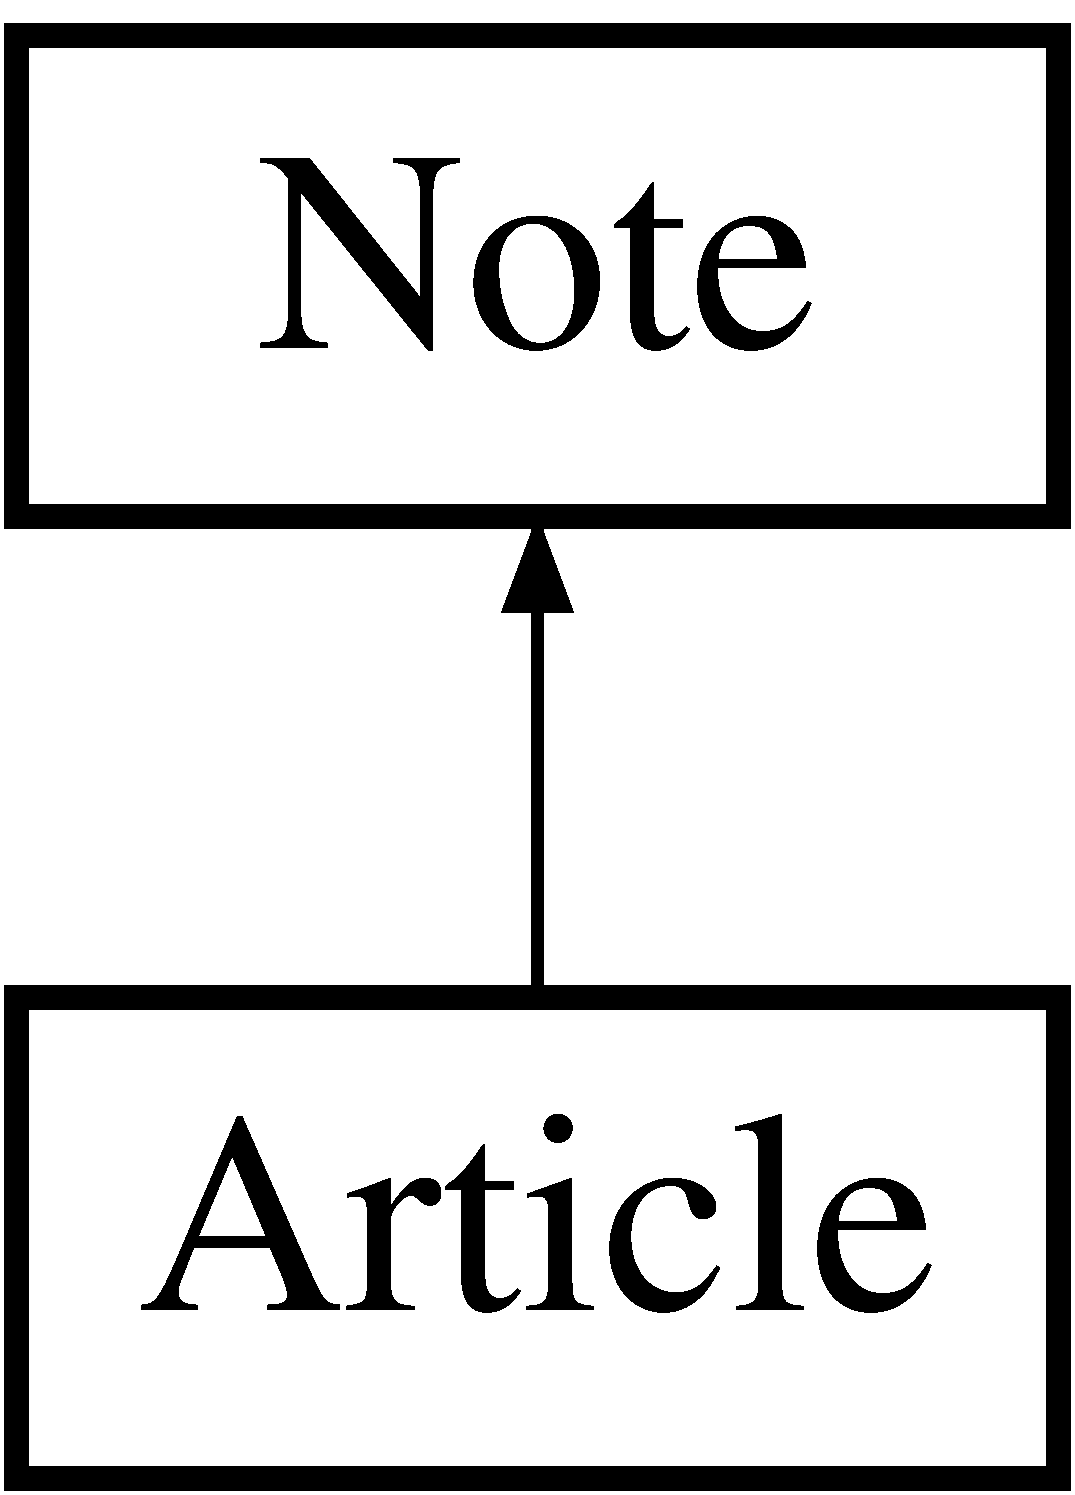
\includegraphics[height=2.000000cm]{classArticle}
\end{center}
\end{figure}
\subsection*{\-Public \-Member \-Functions}
\begin{DoxyCompactItemize}
\item 
\hypertarget{classArticle_a52709bc8511c58d4a7e3c975a42a4c45}{{\bfseries \-Article} (const \-Q\-String \&id, const \-Q\-String \&title, const \-Q\-String \&ctt=\char`\"{}\char`\"{})}\label{classArticle_a52709bc8511c58d4a7e3c975a42a4c45}

\item 
\hypertarget{classArticle_a070b8ab5ea1422f53a50b7ab35ec9a75}{\-Q\-String {\bfseries get\-Content} ()}\label{classArticle_a070b8ab5ea1422f53a50b7ab35ec9a75}

\item 
\hypertarget{classArticle_a5052d0c9a07f637bbbfbc3d0eac4d216}{void {\bfseries set\-Content} (const \-Q\-String \&ctt)}\label{classArticle_a5052d0c9a07f637bbbfbc3d0eac4d216}

\item 
\hypertarget{classArticle_a138e8393aeab078d015e133a71976fc8}{void {\bfseries makehtmlbody} (\-Q\-Xml\-Stream\-Writer $\ast$qw)}\label{classArticle_a138e8393aeab078d015e133a71976fc8}

\item 
\hypertarget{classArticle_ade6e2228c6e152b0f8a76b8a805c772f}{\-Q\-String {\bfseries to\-T\-E\-X} ()}\label{classArticle_ade6e2228c6e152b0f8a76b8a805c772f}

\item 
\hypertarget{classArticle_ae7abb57cd2860a012971498cbb210cb2}{\-Q\-String {\bfseries to\-T\-E\-X\-T} ()}\label{classArticle_ae7abb57cd2860a012971498cbb210cb2}

\item 
\hypertarget{classArticle_abf96d5e7b1841cc629e16e9dbab65fde}{\-Q\-Text\-Stream \& {\bfseries save} (\-Q\-Text\-Stream \&f)}\label{classArticle_abf96d5e7b1841cc629e16e9dbab65fde}

\item 
\hypertarget{classArticle_ac9ed870803a2b86bb3c3e192e310e13d}{\hyperlink{classNoteEditor}{\-Note\-Editor} $\ast$ {\bfseries get\-Editor} (\-Q\-Widget $\ast$parent=\-N\-U\-L\-L)}\label{classArticle_ac9ed870803a2b86bb3c3e192e310e13d}

\end{DoxyCompactItemize}


\subsection{\-Detailed \-Description}
\-Correspond à la spécification de \hyperlink{classNote}{\-Note} pour contenir\-: un article (texte) et des exports \-H\-T\-M\-L,\-Tex,\-T\-E\-X\-T correspondants 

\-The documentation for this class was generated from the following files\-:\begin{DoxyCompactItemize}
\item 
\-Article.\-h\item 
\-Article.\-cpp\end{DoxyCompactItemize}

\hypertarget{classArticleEditor}{\section{\-Article\-Editor \-Class \-Reference}
\label{classArticleEditor}\index{\-Article\-Editor@{\-Article\-Editor}}
}
\-Inheritance diagram for \-Article\-Editor\-:\begin{figure}[H]
\begin{center}
\leavevmode
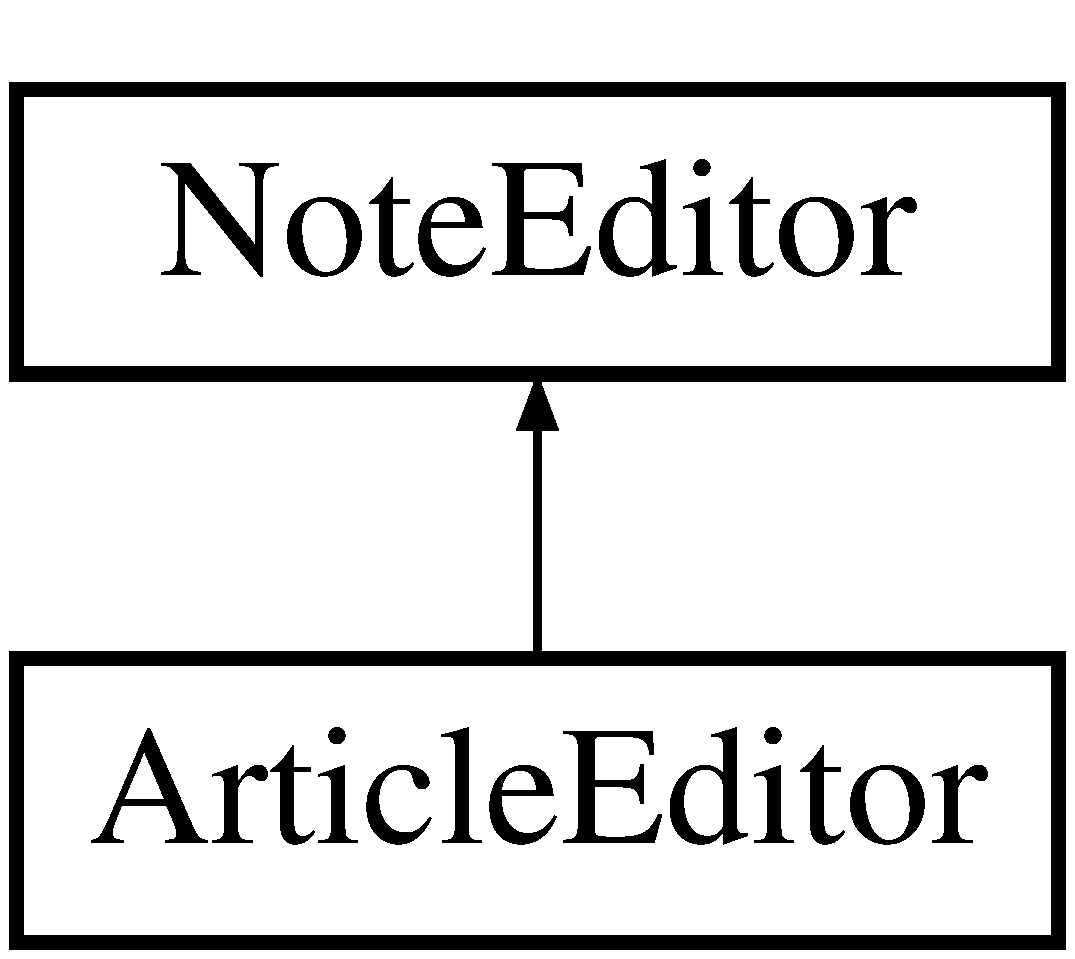
\includegraphics[height=2.000000cm]{classArticleEditor}
\end{center}
\end{figure}
\subsection*{\-Public \-Slots}
\begin{DoxyCompactItemize}
\item 
\hypertarget{classArticleEditor_a859f265d06e8cf80e45e26b1e1d11be4}{void {\bfseries update} (\-Q\-String s=\char`\"{}\char`\"{})}\label{classArticleEditor_a859f265d06e8cf80e45e26b1e1d11be4}

\item 
\hypertarget{classArticleEditor_a2f371197ece3d2e741ae1676748399d8}{void {\bfseries content\-Mod} ()}\label{classArticleEditor_a2f371197ece3d2e741ae1676748399d8}

\end{DoxyCompactItemize}
\subsection*{\-Signals}
\begin{DoxyCompactItemize}
\item 
\hypertarget{classArticleEditor_af7b571d5064e2871eb8905497b538cc6}{void {\bfseries update\-S} (\-Q\-String)}\label{classArticleEditor_af7b571d5064e2871eb8905497b538cc6}

\end{DoxyCompactItemize}
\subsection*{\-Public \-Member \-Functions}
\begin{DoxyCompactItemize}
\item 
\hypertarget{classArticleEditor_a05614b57049ba0db303a571b1a8d516b}{{\bfseries \-Article\-Editor} (\hyperlink{classArticle}{\-Article} $\ast$a, \-Q\-Widget $\ast$parent=0)}\label{classArticleEditor_a05614b57049ba0db303a571b1a8d516b}

\end{DoxyCompactItemize}
\subsection*{\-Protected \-Attributes}
\begin{DoxyCompactItemize}
\item 
\hypertarget{classArticleEditor_afe9ce3d19084c00eda6c783073dd4fa0}{\-Q\-Text\-Edit $\ast$ {\bfseries content}}\label{classArticleEditor_afe9ce3d19084c00eda6c783073dd4fa0}

\end{DoxyCompactItemize}


\-The documentation for this class was generated from the following files\-:\begin{DoxyCompactItemize}
\item 
\-Article.\-h\item 
\-Article.\-cpp\end{DoxyCompactItemize}

\hypertarget{classAudio}{\section{\-Audio \-Class \-Reference}
\label{classAudio}\index{\-Audio@{\-Audio}}
}


{\ttfamily \#include $<$\-Audio.\-h$>$}

\-Inheritance diagram for \-Audio\-:\begin{figure}[H]
\begin{center}
\leavevmode
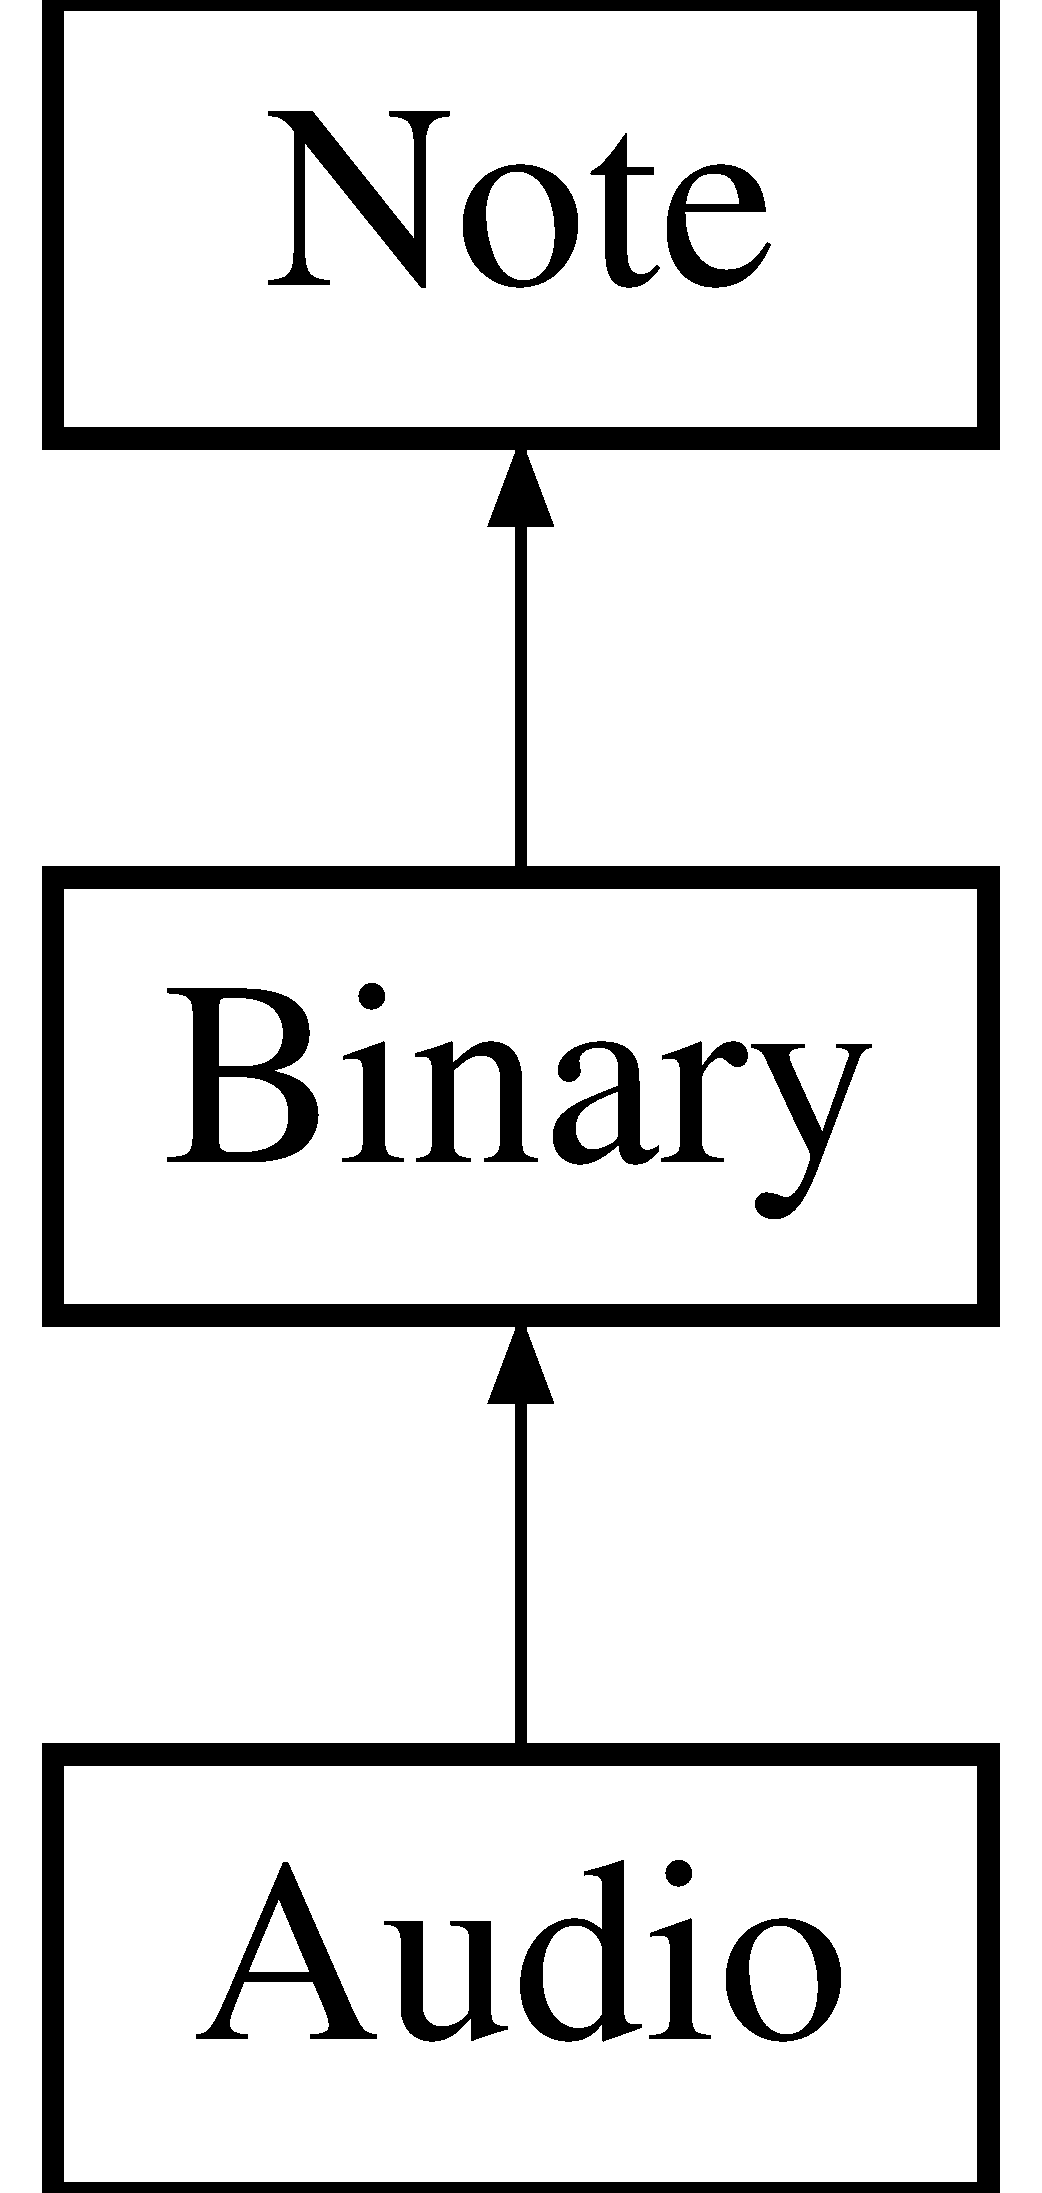
\includegraphics[height=3.000000cm]{classAudio}
\end{center}
\end{figure}
\subsection*{\-Public \-Member \-Functions}
\begin{DoxyCompactItemize}
\item 
\hypertarget{classAudio_af4e17370a77f7d8e3d9cd177b29677a9}{{\bfseries \-Audio} (const \-Q\-String \&id, const \-Q\-String \&title, const \-Q\-String \&desc=\char`\"{}\char`\"{}, const \-Q\-String \&path=\char`\"{}\char`\"{})}\label{classAudio_af4e17370a77f7d8e3d9cd177b29677a9}

\item 
\hypertarget{classAudio_a0dda4963d5d0ad70915483fc9085560b}{void {\bfseries makehtmlbody} (\-Q\-Xml\-Stream\-Writer $\ast$qw)}\label{classAudio_a0dda4963d5d0ad70915483fc9085560b}

\item 
\hypertarget{classAudio_a3018b17d64f9aef97055fd47fbf5d305}{\-Q\-String {\bfseries to\-T\-E\-X} ()}\label{classAudio_a3018b17d64f9aef97055fd47fbf5d305}

\item 
\hypertarget{classAudio_a7919a8446d5ca66c138cf9d0fa70b106}{\-Q\-String {\bfseries to\-T\-E\-X\-T} ()}\label{classAudio_a7919a8446d5ca66c138cf9d0fa70b106}

\item 
\hypertarget{classAudio_aa288d26d55337269d24f2cd01fdabe38}{\-Q\-Text\-Stream \& {\bfseries save} (\-Q\-Text\-Stream \&f)}\label{classAudio_aa288d26d55337269d24f2cd01fdabe38}

\item 
\hypertarget{classAudio_ab7e8bbe8d18afca4002487da748d05f1}{\hyperlink{classNoteEditor}{\-Note\-Editor} $\ast$ {\bfseries get\-Editor} (\-Q\-Widget $\ast$parent=\-N\-U\-L\-L)}\label{classAudio_ab7e8bbe8d18afca4002487da748d05f1}

\end{DoxyCompactItemize}


\subsection{\-Detailed \-Description}
\-Correspond à la spécification de \hyperlink{classBinary}{\-Binary} pour contenir\-: un fichier audio (.wav) et des exports \-H\-T\-M\-L,\-Tex,\-T\-E\-X\-T correspondants 

\-The documentation for this class was generated from the following files\-:\begin{DoxyCompactItemize}
\item 
\-Audio.\-h\item 
\-Audio.\-cpp\end{DoxyCompactItemize}

\hypertarget{classAudioEditor}{\section{\-Audio\-Editor \-Class \-Reference}
\label{classAudioEditor}\index{\-Audio\-Editor@{\-Audio\-Editor}}
}
\-Inheritance diagram for \-Audio\-Editor\-:\begin{figure}[H]
\begin{center}
\leavevmode
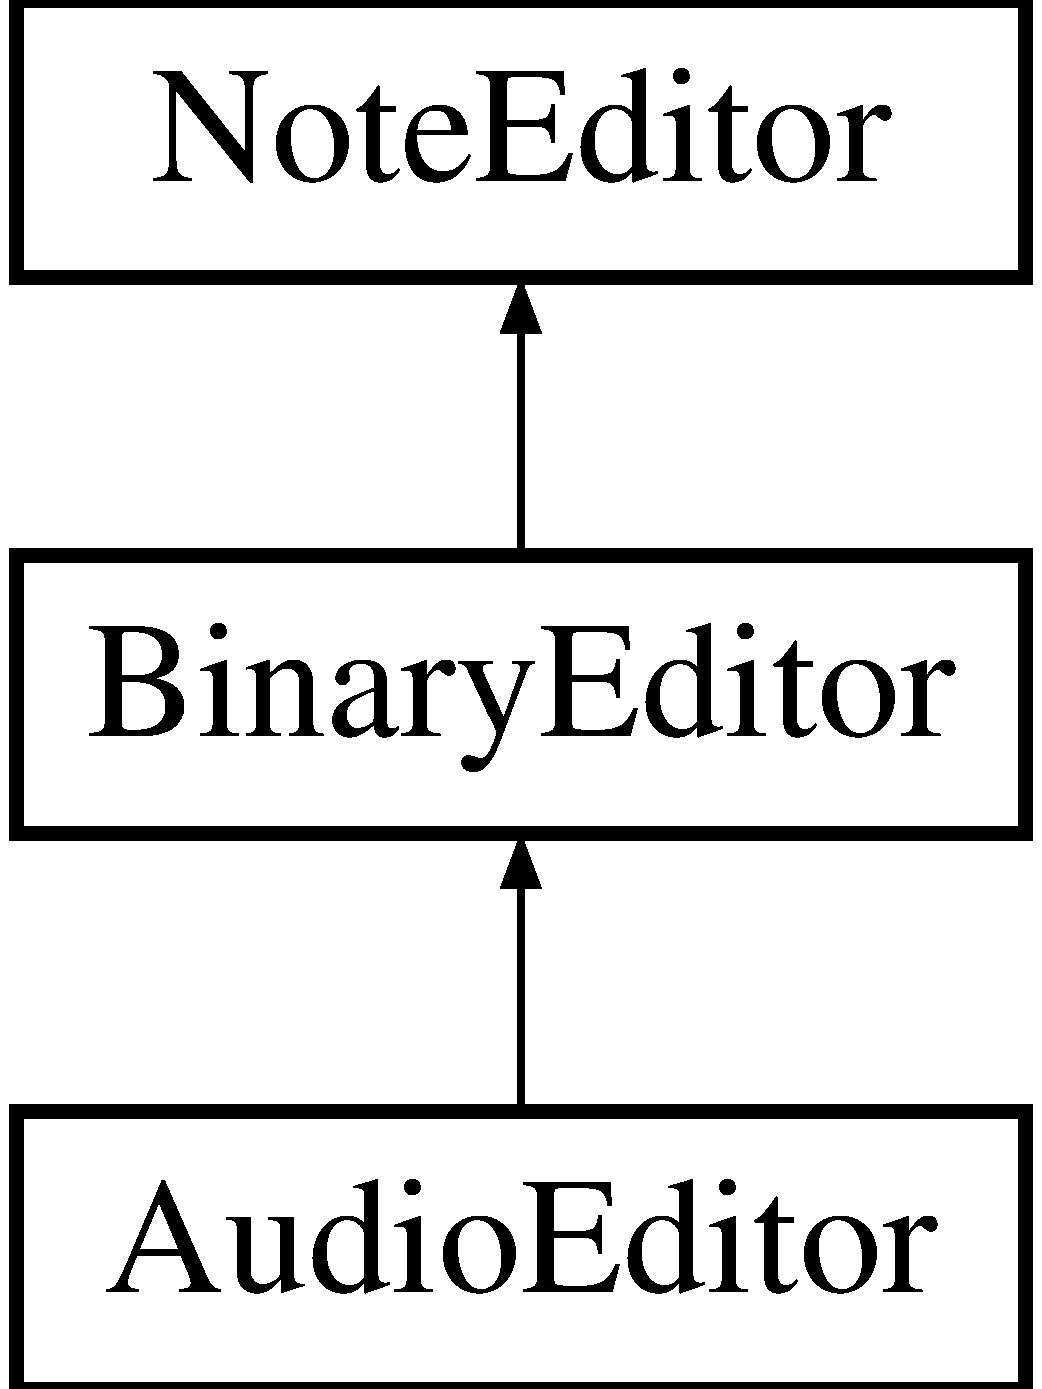
\includegraphics[height=3.000000cm]{classAudioEditor}
\end{center}
\end{figure}
\subsection*{\-Public \-Member \-Functions}
\begin{DoxyCompactItemize}
\item 
\hypertarget{classAudioEditor_acd534b15b2ce58480b0479439e7dd3be}{{\bfseries \-Audio\-Editor} (\hyperlink{classAudio}{\-Audio} $\ast$a, \-Q\-Widget $\ast$parent=0)}\label{classAudioEditor_acd534b15b2ce58480b0479439e7dd3be}

\item 
\hypertarget{classAudioEditor_a03ab5938411b0b8085cd9fc67a77da7b}{\-Q\-String {\bfseries select\-File} ()}\label{classAudioEditor_a03ab5938411b0b8085cd9fc67a77da7b}

\item 
\hypertarget{classAudioEditor_a789f71d54c019cf977e7295dbd647b29}{void {\bfseries update\-Bin} ()}\label{classAudioEditor_a789f71d54c019cf977e7295dbd647b29}

\end{DoxyCompactItemize}


\-The documentation for this class was generated from the following files\-:\begin{DoxyCompactItemize}
\item 
\-Audio.\-h\item 
\-Audio.\-cpp\end{DoxyCompactItemize}

\hypertarget{classBinary}{\section{\-Binary \-Class \-Reference}
\label{classBinary}\index{\-Binary@{\-Binary}}
}
\-Inheritance diagram for \-Binary\-:\begin{figure}[H]
\begin{center}
\leavevmode
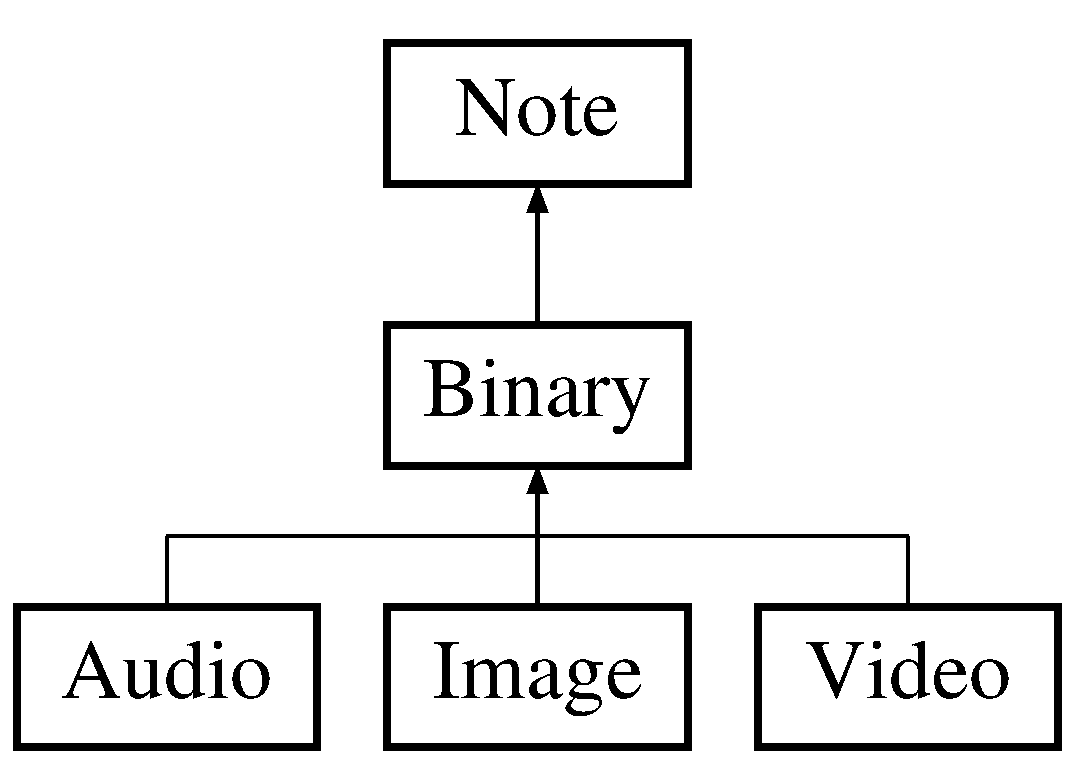
\includegraphics[height=3.000000cm]{classBinary}
\end{center}
\end{figure}
\subsection*{\-Public \-Member \-Functions}
\begin{DoxyCompactItemize}
\item 
\hypertarget{classBinary_a8f8e5cf0c64bc1c1cc1bc2b9e7e3cfe2}{{\bfseries \-Binary} (const \-Q\-String \&type, const \-Q\-String \&id, const \-Q\-String \&title, const \-Q\-String \&d, const \-Q\-String \&p)}\label{classBinary_a8f8e5cf0c64bc1c1cc1bc2b9e7e3cfe2}

\item 
\hypertarget{classBinary_a1c69ab4bffa479268f5e76a5f9ea2239}{\-Q\-String \& {\bfseries get\-Desc} ()}\label{classBinary_a1c69ab4bffa479268f5e76a5f9ea2239}

\item 
\hypertarget{classBinary_a1cbb14af940b5ae61887dc9931f1c914}{void {\bfseries set\-Desc} (const \-Q\-String \&d)}\label{classBinary_a1cbb14af940b5ae61887dc9931f1c914}

\item 
\hypertarget{classBinary_a2e9e439c4f6dfd9ad8c934ee1770956d}{\-Q\-String \& {\bfseries get\-Path} ()}\label{classBinary_a2e9e439c4f6dfd9ad8c934ee1770956d}

\item 
\hypertarget{classBinary_af564f148d20972efabb9c84357a40b58}{void {\bfseries set\-Path} (const \-Q\-String \&p)}\label{classBinary_af564f148d20972efabb9c84357a40b58}

\item 
\hypertarget{classBinary_a6c4838210e5b73ace50a931b3fddd0b2}{virtual \-Q\-Text\-Stream \& {\bfseries save} (\-Q\-Text\-Stream \&f)=0}\label{classBinary_a6c4838210e5b73ace50a931b3fddd0b2}

\item 
\hypertarget{classBinary_af9d27a0059a8fc7dc20c5497eda548ac}{virtual \hyperlink{classNoteEditor}{\-Note\-Editor} $\ast$ {\bfseries get\-Editor} (\-Q\-Widget $\ast$parent=\-N\-U\-L\-L)=0}\label{classBinary_af9d27a0059a8fc7dc20c5497eda548ac}

\item 
\hypertarget{classBinary_ab2e81910a027eefdbd14c11ea3ef2d31}{virtual \-Q\-String {\bfseries to\-T\-E\-X} ()=0}\label{classBinary_ab2e81910a027eefdbd14c11ea3ef2d31}

\item 
\hypertarget{classBinary_a0571d2774b66b5ccbb60aecfb9b111d1}{virtual \-Q\-String {\bfseries to\-T\-E\-X\-T} ()=0}\label{classBinary_a0571d2774b66b5ccbb60aecfb9b111d1}

\item 
\hypertarget{classBinary_a1d6197854ccf7b1fcdce3a11bc9c1a37}{virtual void {\bfseries makehtmlbody} (\-Q\-Xml\-Stream\-Writer $\ast$qw)}\label{classBinary_a1d6197854ccf7b1fcdce3a11bc9c1a37}

\end{DoxyCompactItemize}
\subsection*{\-Protected \-Member \-Functions}
\begin{DoxyCompactItemize}
\item 
\hypertarget{classBinary_a91c7ab94c9a90378d050c647a3b828ae}{{\bfseries \-Binary} (\hyperlink{classBinary}{\-Binary} \&b)}\label{classBinary_a91c7ab94c9a90378d050c647a3b828ae}

\item 
\hypertarget{classBinary_a63012d4e15470cc40cced167575be9b7}{void {\bfseries operator=} (const \hyperlink{classBinary}{\-Binary} \&b)}\label{classBinary_a63012d4e15470cc40cced167575be9b7}

\item 
\hypertarget{classBinary_a20cf14022913ce26fbb3b0fd59c7fccf}{virtual void {\bfseries load} ()=0}\label{classBinary_a20cf14022913ce26fbb3b0fd59c7fccf}

\end{DoxyCompactItemize}
\subsection*{\-Protected \-Attributes}
\begin{DoxyCompactItemize}
\item 
\hypertarget{classBinary_ac1f3c9e3488d40f6d08be99f33a537db}{\-Q\-String {\bfseries desc}}\label{classBinary_ac1f3c9e3488d40f6d08be99f33a537db}

\item 
\hypertarget{classBinary_ae7a554907a63301507ee154ddaed9d56}{\-Q\-String {\bfseries path}}\label{classBinary_ae7a554907a63301507ee154ddaed9d56}

\end{DoxyCompactItemize}


\subsection{\-Detailed \-Description}
\-Correspond à la spécification de \hyperlink{classNote}{\-Note} pour contenir\-: un fichier binaire une description un \-Path( chemin d'accès) un type d'éditeur i.\-e. un graphisme spécifique 

\-The documentation for this class was generated from the following files\-:\begin{DoxyCompactItemize}
\item 
\-Binary.\-h\item 
\-Binary.\-cpp\end{DoxyCompactItemize}

\hypertarget{classBinaryEditor}{\section{\-Binary\-Editor \-Class \-Reference}
\label{classBinaryEditor}\index{\-Binary\-Editor@{\-Binary\-Editor}}
}
\-Inheritance diagram for \-Binary\-Editor\-:\begin{figure}[H]
\begin{center}
\leavevmode
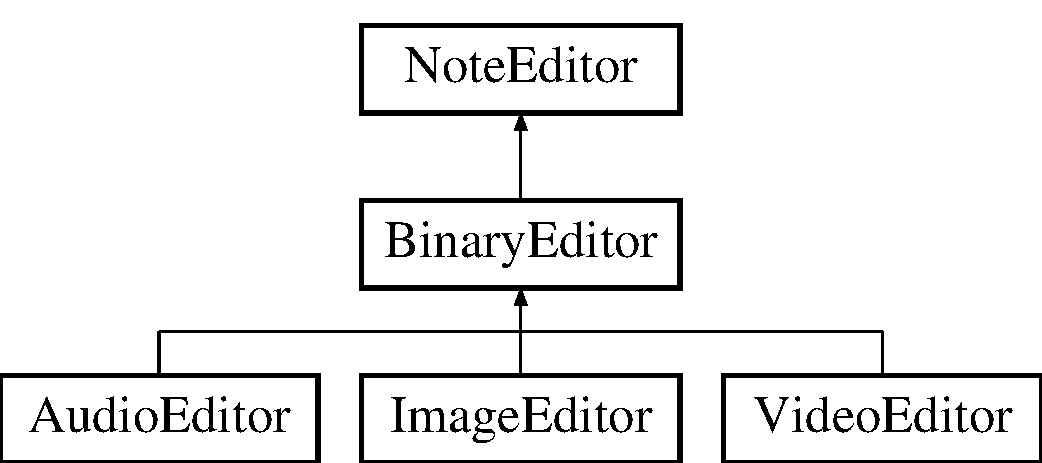
\includegraphics[height=3.000000cm]{classBinaryEditor}
\end{center}
\end{figure}
\subsection*{\-Public \-Slots}
\begin{DoxyCompactItemize}
\item 
\hypertarget{classBinaryEditor_a2d70480e4b7b1f4e6db2d7ff3f5d09c2}{void {\bfseries change\-File} ()}\label{classBinaryEditor_a2d70480e4b7b1f4e6db2d7ff3f5d09c2}

\item 
\hypertarget{classBinaryEditor_add18586342bbdc59cfadf4333e67d3e4}{void {\bfseries desc\-Mod} ()}\label{classBinaryEditor_add18586342bbdc59cfadf4333e67d3e4}

\end{DoxyCompactItemize}
\subsection*{\-Public \-Member \-Functions}
\begin{DoxyCompactItemize}
\item 
\hypertarget{classBinaryEditor_ab417e9c2a932d10cfdfa98db1493c0cf}{{\bfseries \-Binary\-Editor} (\hyperlink{classBinary}{\-Binary} $\ast$b, \-Q\-Widget $\ast$parent=0)}\label{classBinaryEditor_ab417e9c2a932d10cfdfa98db1493c0cf}

\item 
\hypertarget{classBinaryEditor_a48623d75859581b4f981a4e33cae314b}{virtual \-Q\-String {\bfseries select\-File} ()=0}\label{classBinaryEditor_a48623d75859581b4f981a4e33cae314b}

\item 
\hypertarget{classBinaryEditor_a14e70913a4e914b02029ae9fd737fcce}{virtual void {\bfseries update\-Bin} ()=0}\label{classBinaryEditor_a14e70913a4e914b02029ae9fd737fcce}

\end{DoxyCompactItemize}
\subsection*{\-Protected \-Attributes}
\begin{DoxyCompactItemize}
\item 
\hypertarget{classBinaryEditor_adb862f876130ef1677d7e62c9b72975e}{\-Q\-Text\-Edit $\ast$ {\bfseries desc}}\label{classBinaryEditor_adb862f876130ef1677d7e62c9b72975e}

\item 
\hypertarget{classBinaryEditor_a8212299c7c02322823bf1b15f91f9383}{\-Q\-Widget $\ast$ {\bfseries path\-Zone}}\label{classBinaryEditor_a8212299c7c02322823bf1b15f91f9383}

\item 
\hypertarget{classBinaryEditor_a86cbd1cb540429e107a6c93190f2801c}{\-Q\-Push\-Button $\ast$ {\bfseries ch\-Path}}\label{classBinaryEditor_a86cbd1cb540429e107a6c93190f2801c}

\item 
\hypertarget{classBinaryEditor_aa7fccc22edc7c9fa3d4af41aa58cc6aa}{\-Q\-Label $\ast$ {\bfseries path}}\label{classBinaryEditor_aa7fccc22edc7c9fa3d4af41aa58cc6aa}

\item 
\hypertarget{classBinaryEditor_a2c0119a9c6525e35ebf52cb8a8f3f9da}{\-Q\-H\-Box\-Layout $\ast$ {\bfseries path\-Lay}}\label{classBinaryEditor_a2c0119a9c6525e35ebf52cb8a8f3f9da}

\end{DoxyCompactItemize}


\-The documentation for this class was generated from the following files\-:\begin{DoxyCompactItemize}
\item 
\-Binary.\-h\item 
\-Binary.\-cpp\end{DoxyCompactItemize}

\hypertarget{classConfig}{\section{\-Config \-Class \-Reference}
\label{classConfig}\index{\-Config@{\-Config}}
}


{\ttfamily \#include $<$\-Config.\-h$>$}

\subsection*{\-Public \-Member \-Functions}
\begin{DoxyCompactItemize}
\item 
\hypertarget{classConfig_aa671501a3bd9abc615dd2336256834ba}{bool {\bfseries is\-W\-S} (const \-Q\-String \&)}\label{classConfig_aa671501a3bd9abc615dd2336256834ba}

\item 
\hypertarget{classConfig_a09b007f6a73298d418c4827a6d9ed935}{unsigned int {\bfseries nb\-W\-S} ()}\label{classConfig_a09b007f6a73298d418c4827a6d9ed935}

\item 
\hypertarget{classConfig_a9a2b5c7f56ae9c8332631b075cf66ecc}{\-Q\-String {\bfseries last\-W\-S} ()}\label{classConfig_a9a2b5c7f56ae9c8332631b075cf66ecc}

\item 
\hypertarget{classConfig_a5274a8150fda0e3f42c436c4addae082}{void {\bfseries update\-Last\-W\-S} (const \-Q\-String \&)}\label{classConfig_a5274a8150fda0e3f42c436c4addae082}

\item 
\hypertarget{classConfig_a2d04091f571813bab7171cf713917aff}{void {\bfseries check} ()}\label{classConfig_a2d04091f571813bab7171cf713917aff}

\item 
\hypertarget{classConfig_aea1c0e81b837e3afc951d1636df8baec}{bool {\bfseries new\-W\-S} (const \-Q\-String \&)}\label{classConfig_aea1c0e81b837e3afc951d1636df8baec}

\item 
\hypertarget{classConfig_af4a8f10b899329e3b804e346fd303ac5}{bool {\bfseries clone\-W\-S} (const \-Q\-String \&, const \-Q\-String \&)}\label{classConfig_af4a8f10b899329e3b804e346fd303ac5}

\item 
\hypertarget{classConfig_ab658ef4d4ec727d7e3e865fb1665611a}{void {\bfseries delete\-W\-S} (const \-Q\-String \&)}\label{classConfig_ab658ef4d4ec727d7e3e865fb1665611a}

\item 
\hypertarget{classConfig_a20ca0832e5cc6c20fb1fedf5464d1b7c}{void {\bfseries update\-Config} ()}\label{classConfig_a20ca0832e5cc6c20fb1fedf5464d1b7c}

\item 
\hypertarget{classConfig_a328b9ebe89ccaa52f0f8732191c8a28a}{\-Q\-List$<$ \-Q\-String $>$ {\bfseries list\-W\-S} ()}\label{classConfig_a328b9ebe89ccaa52f0f8732191c8a28a}

\end{DoxyCompactItemize}


\subsection{\-Detailed \-Description}
un \-Path( chemin d'accès) un type d'éditeur i.\-e. un graphisme spécifique

\-Gère le fichier de configuration du programme avec\-: les différents \-Workspaces les opérations sur ceux-\/ci 

\-The documentation for this class was generated from the following files\-:\begin{DoxyCompactItemize}
\item 
\-Config.\-h\item 
\-Config.\-cpp\end{DoxyCompactItemize}

\hypertarget{classConfigManager}{\section{\-Config\-Manager \-Class \-Reference}
\label{classConfigManager}\index{\-Config\-Manager@{\-Config\-Manager}}
}
\subsection*{\-Public \-Slots}
\begin{DoxyCompactItemize}
\item 
\hypertarget{classConfigManager_a721c4c7e71713002bcadf57b4883fae3}{void {\bfseries safe\-Del} ()}\label{classConfigManager_a721c4c7e71713002bcadf57b4883fae3}

\item 
\hypertarget{classConfigManager_a74c86eb13b1deda508a0483e41b026a9}{void {\bfseries del\-W\-S} ()}\label{classConfigManager_a74c86eb13b1deda508a0483e41b026a9}

\item 
\hypertarget{classConfigManager_a43b9c7671430720e150968e46a176aa4}{void {\bfseries new\-W\-S} ()}\label{classConfigManager_a43b9c7671430720e150968e46a176aa4}

\item 
\hypertarget{classConfigManager_a00d1376c8bc83c2d8962fcd425f9ab41}{void {\bfseries clone\-W\-S} ()}\label{classConfigManager_a00d1376c8bc83c2d8962fcd425f9ab41}

\item 
\hypertarget{classConfigManager_a2bebbaeb585436602c80979000e3b774}{void {\bfseries load\-W\-S} ()}\label{classConfigManager_a2bebbaeb585436602c80979000e3b774}

\item 
\hypertarget{classConfigManager_aeaa86a9dc608bc9b12cbc40348a07f27}{void {\bfseries show\-Notes} (\-Q\-List\-Widget\-Item $\ast$)}\label{classConfigManager_aeaa86a9dc608bc9b12cbc40348a07f27}

\end{DoxyCompactItemize}
\subsection*{\-Public \-Member \-Functions}
\begin{DoxyCompactItemize}
\item 
\hypertarget{classConfigManager_a58aa03db1b1215570423961a53aeea63}{{\bfseries \-Config\-Manager} (\-Q\-Widget $\ast$parent=\-N\-U\-L\-L)}\label{classConfigManager_a58aa03db1b1215570423961a53aeea63}

\item 
\hypertarget{classConfigManager_af1f8eeb720a79a591f2aa12de3abb458}{\-Q\-String {\bfseries get\-Path} () const }\label{classConfigManager_af1f8eeb720a79a591f2aa12de3abb458}

\item 
\hypertarget{classConfigManager_a49a873f13e89fbae0e0f74ea0a18f7ee}{void {\bfseries update\-G\-U\-I} ()}\label{classConfigManager_a49a873f13e89fbae0e0f74ea0a18f7ee}

\end{DoxyCompactItemize}


\-The documentation for this class was generated from the following files\-:\begin{DoxyCompactItemize}
\item 
\-Config.\-h\item 
\-Config.\-cpp\end{DoxyCompactItemize}

\hypertarget{classDocButton}{\section{\-Doc\-Button \-Class \-Reference}
\label{classDocButton}\index{\-Doc\-Button@{\-Doc\-Button}}
}
\subsection*{\-Public \-Slots}
\begin{DoxyCompactItemize}
\item 
\hypertarget{classDocButton_a5d63f4e51ca56ab7baf5889e48e15a18}{void {\bfseries get\-Wid} ()}\label{classDocButton_a5d63f4e51ca56ab7baf5889e48e15a18}

\end{DoxyCompactItemize}
\subsection*{\-Signals}
\begin{DoxyCompactItemize}
\item 
\hypertarget{classDocButton_abcd0d83f0fa7b5fa65a77bad45440641}{void {\bfseries send\-Wid} (\-Q\-Widget $\ast$)}\label{classDocButton_abcd0d83f0fa7b5fa65a77bad45440641}

\end{DoxyCompactItemize}
\subsection*{\-Public \-Member \-Functions}
\begin{DoxyCompactItemize}
\item 
\hypertarget{classDocButton_abbf6712177714850a283ab7ac9699232}{{\bfseries \-Doc\-Button} (\-Q\-Widget $\ast$wid, const \-Q\-Icon \&ico, const \-Q\-String \&txt, \-Q\-Widget $\ast$p=\-N\-U\-L\-L)}\label{classDocButton_abbf6712177714850a283ab7ac9699232}

\item 
\hypertarget{classDocButton_a6a3dba7215d7ccd3d0d845d6caaa74bf}{{\bfseries \-Doc\-Button} (\-Q\-Widget $\ast$wid, const \-Q\-String \&txt, \-Q\-Widget $\ast$p=\-N\-U\-L\-L)}\label{classDocButton_a6a3dba7215d7ccd3d0d845d6caaa74bf}

\end{DoxyCompactItemize}


\-The documentation for this class was generated from the following files\-:\begin{DoxyCompactItemize}
\item 
\-Document.\-h\item 
\-Document.\-cpp\end{DoxyCompactItemize}

\hypertarget{classDocument}{\section{\-Document \-Class \-Reference}
\label{classDocument}\index{\-Document@{\-Document}}
}


{\ttfamily \#include $<$\-Document.\-h$>$}

\-Inheritance diagram for \-Document\-:\begin{figure}[H]
\begin{center}
\leavevmode
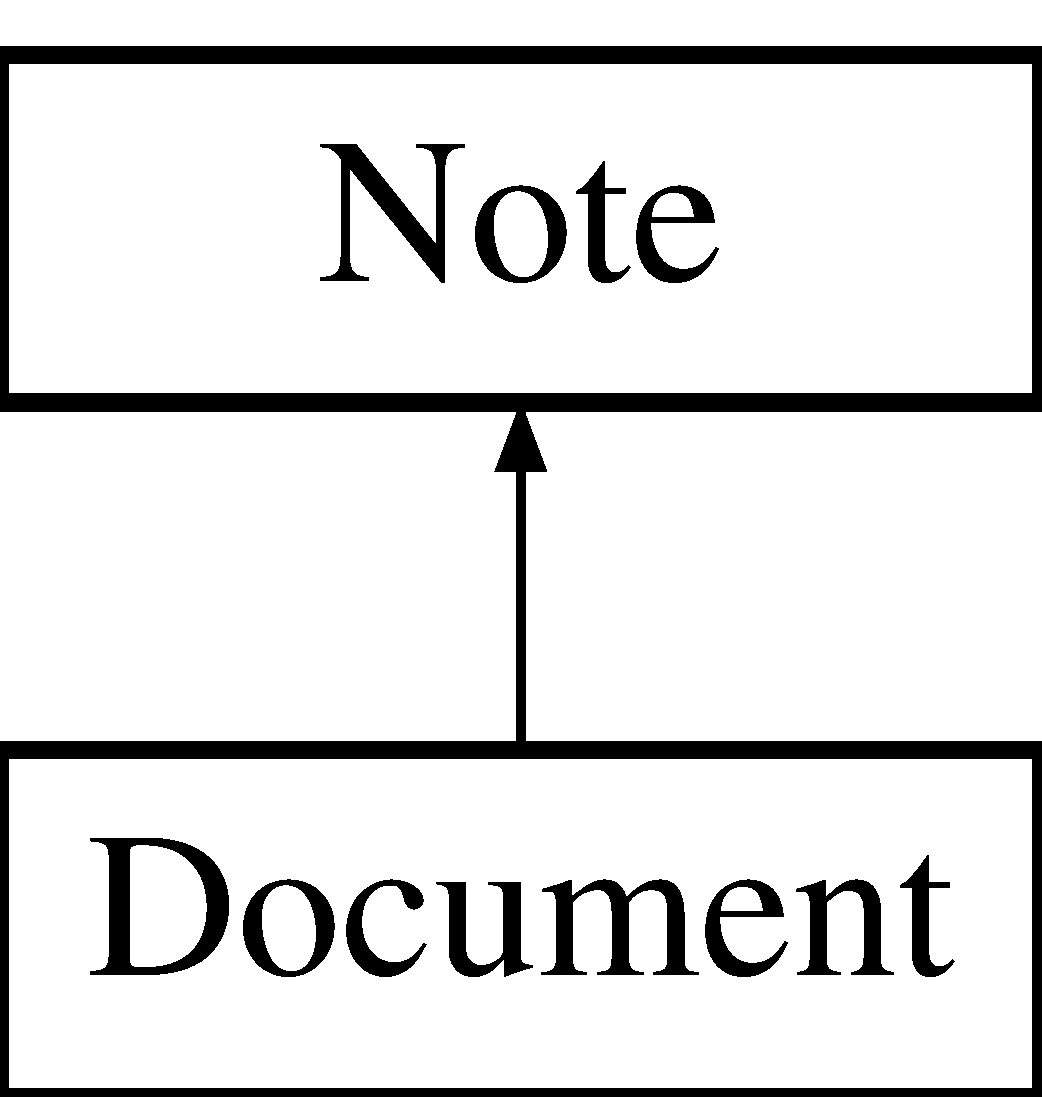
\includegraphics[height=2.000000cm]{classDocument}
\end{center}
\end{figure}
\subsection*{\-Public \-Member \-Functions}
\begin{DoxyCompactItemize}
\item 
\hypertarget{classDocument_a981b6426029d44d63384548cb347ea9f}{{\bfseries \-Document} (const \-Q\-String \&id, const \-Q\-String \&title, const std\-::list$<$ \hyperlink{classNote}{\-Note} $\ast$ $>$ content=std\-::list$<$ \hyperlink{classNote}{\-Note} $\ast$ $>$())}\label{classDocument_a981b6426029d44d63384548cb347ea9f}

\item 
\hypertarget{classDocument_a497e0d38a648361bbc5f9e8eb6da04a7}{void {\bfseries add\-Sub\-Note} (\hyperlink{classNote}{\-Note} $\ast$n)}\label{classDocument_a497e0d38a648361bbc5f9e8eb6da04a7}

\item 
\hypertarget{classDocument_a9bd7efe91c8d6e7d7076b1abf0b066fb}{void {\bfseries add\-Sub\-Note} (\hyperlink{classNote}{\-Note} $\ast$n, unsigned int)}\label{classDocument_a9bd7efe91c8d6e7d7076b1abf0b066fb}

\item 
\hypertarget{classDocument_a66a3b9b6cb032fdafc7eb279d2c87966}{void {\bfseries remove\-Sub\-Note} (unsigned int)}\label{classDocument_a66a3b9b6cb032fdafc7eb279d2c87966}

\item 
\hypertarget{classDocument_a4c718cf328450937d10e8c355d3b6422}{void {\bfseries remove\-Sub\-Note} (const \hyperlink{classNote}{\-Note} $\ast$)}\label{classDocument_a4c718cf328450937d10e8c355d3b6422}

\item 
\hypertarget{classDocument_a0d28a68344f71d71c44b6f5ef27b97cb}{\hyperlink{classNote}{\-Note} $\ast$ {\bfseries get\-Sub\-Note} (unsigned int pos)}\label{classDocument_a0d28a68344f71d71c44b6f5ef27b97cb}

\item 
\hypertarget{classDocument_aeea96bc9cb8575b90cb6508622746e5a}{bool {\bfseries is\-Note} (const \hyperlink{classNote}{\-Note} $\ast$)}\label{classDocument_aeea96bc9cb8575b90cb6508622746e5a}

\item 
\hypertarget{classDocument_abd1b2179b00d843932abf4aef2b1d07e}{bool {\bfseries is\-Note} (const \-Q\-String \&)}\label{classDocument_abd1b2179b00d843932abf4aef2b1d07e}

\item 
\hypertarget{classDocument_ae61276d28ebbc3ceb5f91907e226868f}{unsigned int {\bfseries get\-Nb\-Sub\-Notes} ()}\label{classDocument_ae61276d28ebbc3ceb5f91907e226868f}

\item 
\hypertarget{classDocument_afeeecb69d4ed6095ffd0b06881d6417c}{\-Q\-Text\-Stream \& {\bfseries save} (\-Q\-Text\-Stream \&f)}\label{classDocument_afeeecb69d4ed6095ffd0b06881d6417c}

\item 
\hypertarget{classDocument_a3fbc8eb1a50ec40c7cd74e5a969921a6}{\hyperlink{classNoteEditor}{\-Note\-Editor} $\ast$ {\bfseries get\-Editor} (\-Q\-Widget $\ast$parent=\-N\-U\-L\-L)}\label{classDocument_a3fbc8eb1a50ec40c7cd74e5a969921a6}

\item 
\hypertarget{classDocument_aeca93d0a046ccf87ff54daa56ea4fbcc}{virtual void {\bfseries makehtmlbody} (\-Q\-Xml\-Stream\-Writer $\ast$qw)}\label{classDocument_aeca93d0a046ccf87ff54daa56ea4fbcc}

\item 
\hypertarget{classDocument_abfe8c70f4db8563d41b1fed8ddbe268c}{\-Q\-String {\bfseries to\-T\-E\-X} ()}\label{classDocument_abfe8c70f4db8563d41b1fed8ddbe268c}

\item 
\hypertarget{classDocument_a47012344c13c7b6f43cce93d23e5f636}{\-Q\-String {\bfseries to\-T\-E\-X\-T} ()}\label{classDocument_a47012344c13c7b6f43cce93d23e5f636}

\end{DoxyCompactItemize}


\subsection{\-Detailed \-Description}
\-Correspond à la spécification de \hyperlink{classNote}{\-Note} pour contenir\-: des sous-\/notes (\hyperlink{classAudio}{\-Audio}, \hyperlink{classArticle}{\-Article}, \hyperlink{classImage}{\-Image}, \hyperlink{classVideo}{\-Video}) un type d'éditeur i.\-e. un graphisme spécifique et des exports \-H\-T\-M\-L,\-Tex,\-T\-E\-X\-T correspondants 

\-The documentation for this class was generated from the following files\-:\begin{DoxyCompactItemize}
\item 
\-Document.\-h\item 
\-Document.\-cpp\end{DoxyCompactItemize}

\hypertarget{classDocumentEditor}{\section{\-Document\-Editor \-Class \-Reference}
\label{classDocumentEditor}\index{\-Document\-Editor@{\-Document\-Editor}}
}
\-Inheritance diagram for \-Document\-Editor\-:\begin{figure}[H]
\begin{center}
\leavevmode
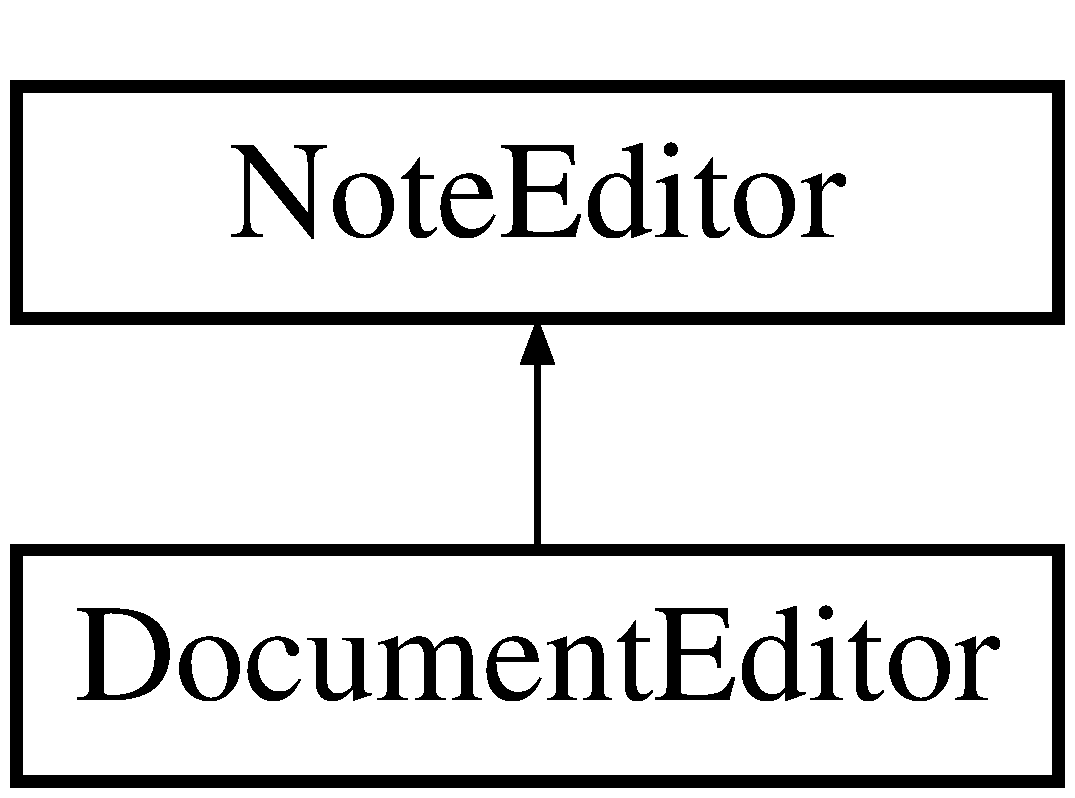
\includegraphics[height=2.000000cm]{classDocumentEditor}
\end{center}
\end{figure}
\subsection*{\-Public \-Slots}
\begin{DoxyCompactItemize}
\item 
\hypertarget{classDocumentEditor_a60c1c8cd663639290a501cc39c251b19}{void {\bfseries detach\-Note} (\-Q\-Widget $\ast$)}\label{classDocumentEditor_a60c1c8cd663639290a501cc39c251b19}

\item 
\hypertarget{classDocumentEditor_a9e770766f29b660cf9e92a17d4566160}{void {\bfseries select\-Note} ()}\label{classDocumentEditor_a9e770766f29b660cf9e92a17d4566160}

\item 
\hypertarget{classDocumentEditor_ae2dcc2a001ced712679623726dfab6ba}{void {\bfseries open\-Note} (\hyperlink{classQListEditorItem}{\-Q\-List\-Editor\-Item} $\ast$)}\label{classDocumentEditor_ae2dcc2a001ced712679623726dfab6ba}

\end{DoxyCompactItemize}
\subsection*{\-Public \-Member \-Functions}
\begin{DoxyCompactItemize}
\item 
\hypertarget{classDocumentEditor_a01dd7e801b855544b12d7b19f5bb86f0}{{\bfseries \-Document\-Editor} (\hyperlink{classDocument}{\-Document} $\ast$d, \-Q\-Widget $\ast$parent=\-N\-U\-L\-L)}\label{classDocumentEditor_a01dd7e801b855544b12d7b19f5bb86f0}

\item 
\hypertarget{classDocumentEditor_ad665510a938c917752d29d59750a2a7b}{void {\bfseries insert\-Note} (\hyperlink{classNoteEditor}{\-Note\-Editor} $\ast$, \-Q\-Widget $\ast$parent=\-N\-U\-L\-L)}\label{classDocumentEditor_ad665510a938c917752d29d59750a2a7b}

\end{DoxyCompactItemize}
\subsection*{\-Protected \-Attributes}
\begin{DoxyCompactItemize}
\item 
\hypertarget{classDocumentEditor_a2a21804611f483b627f3ed7cdaf3c793}{std\-::list$<$ \-Q\-Widget $\ast$ $>$ {\bfseries content}}\label{classDocumentEditor_a2a21804611f483b627f3ed7cdaf3c793}

\item 
\hypertarget{classDocumentEditor_ab27ebe3a03ae68be4dfdaf33bdfa04b8}{\-Q\-Dialog $\ast$ {\bfseries ask}}\label{classDocumentEditor_ab27ebe3a03ae68be4dfdaf33bdfa04b8}

\item 
\hypertarget{classDocumentEditor_aa8efcc8f9e9a9b1456042ce1ab3b1f4f}{\hyperlink{classQListEditor}{\-Q\-List\-Editor} $\ast$ {\bfseries notes}}\label{classDocumentEditor_aa8efcc8f9e9a9b1456042ce1ab3b1f4f}

\end{DoxyCompactItemize}


\-The documentation for this class was generated from the following files\-:\begin{DoxyCompactItemize}
\item 
\-Document.\-h\item 
\-Document.\-cpp\end{DoxyCompactItemize}

\hypertarget{classImage}{\section{\-Image \-Class \-Reference}
\label{classImage}\index{\-Image@{\-Image}}
}


{\ttfamily \#include $<$\-Image.\-h$>$}

\-Inheritance diagram for \-Image\-:\begin{figure}[H]
\begin{center}
\leavevmode
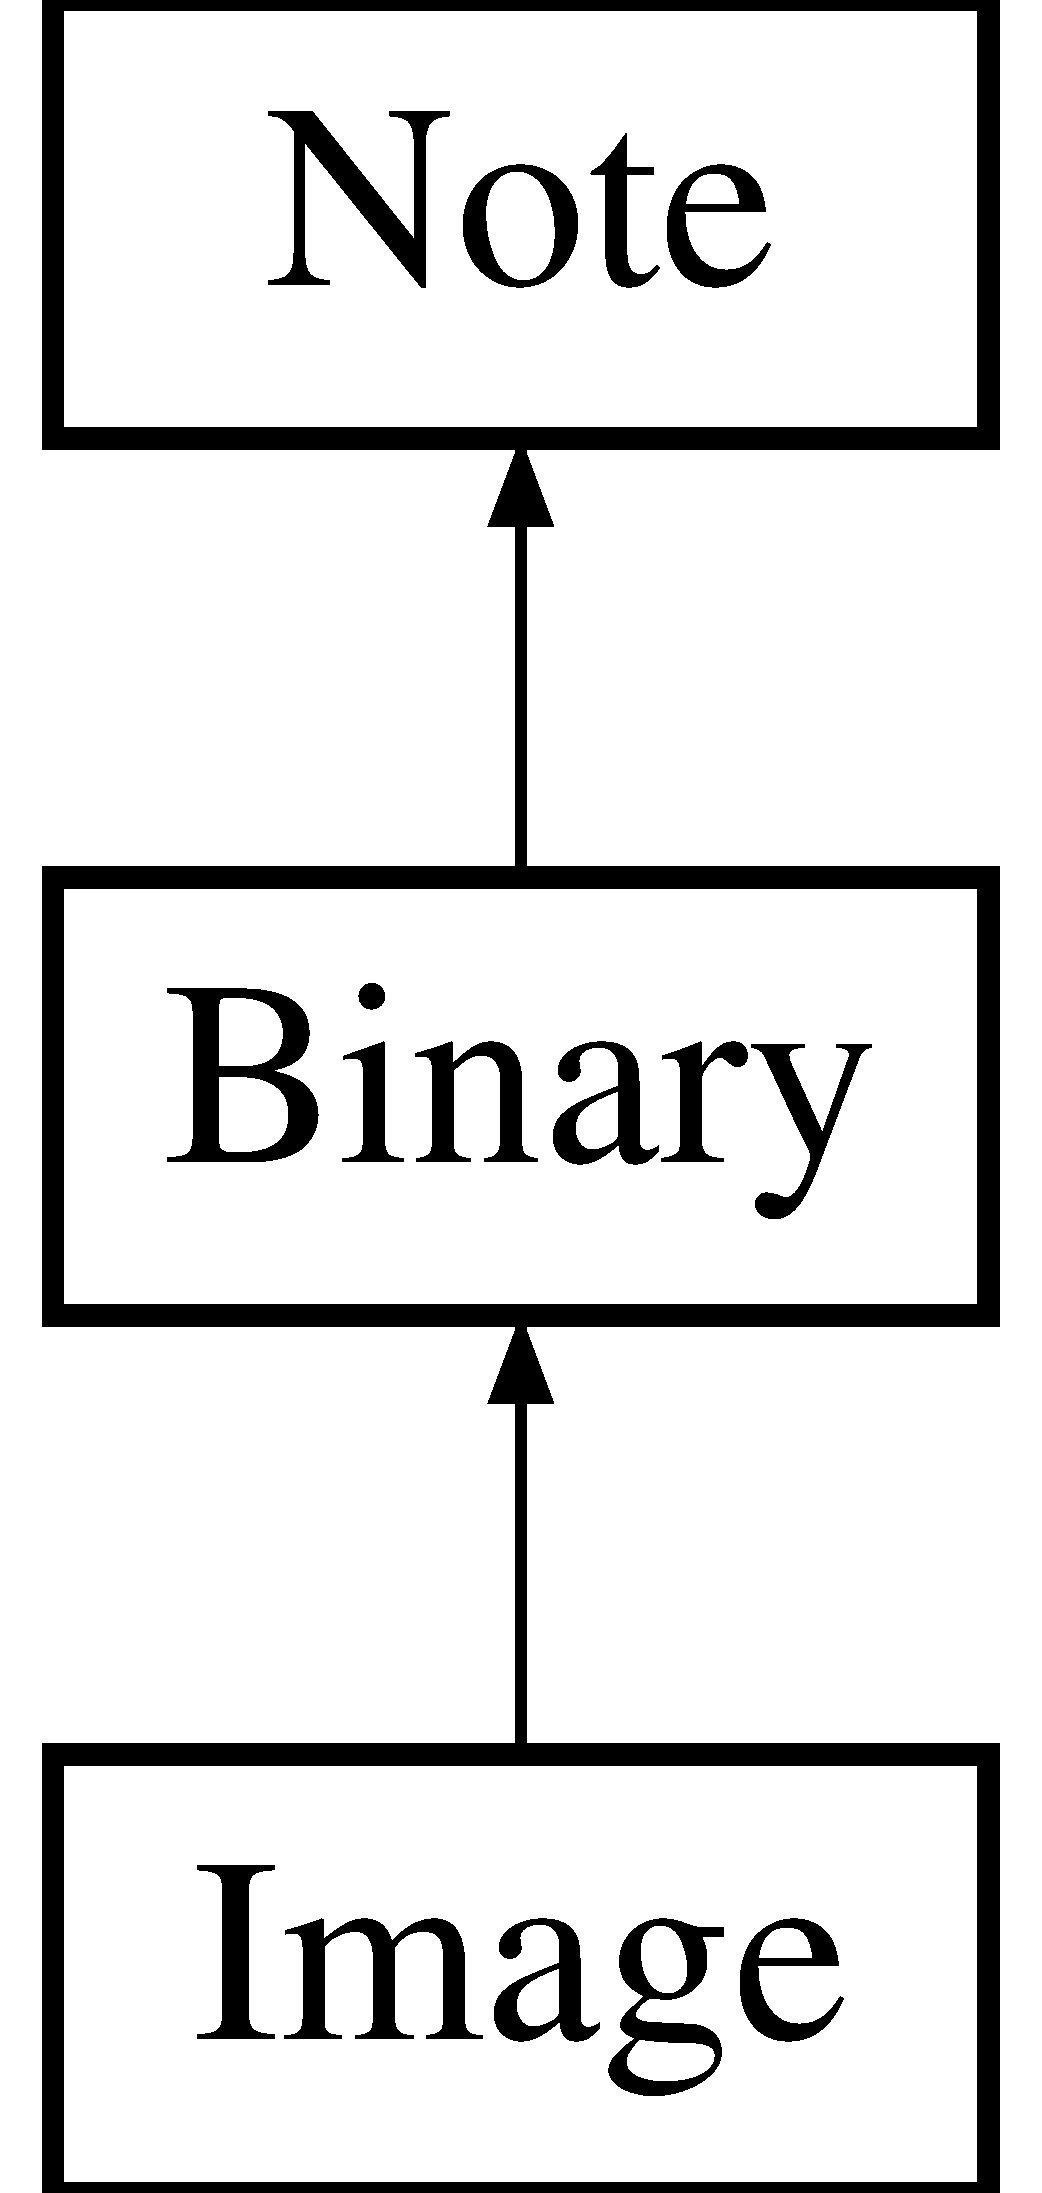
\includegraphics[height=3.000000cm]{classImage}
\end{center}
\end{figure}
\subsection*{\-Public \-Member \-Functions}
\begin{DoxyCompactItemize}
\item 
\hypertarget{classImage_ad8352740e64313fd59ecb27f814a2c11}{{\bfseries \-Image} (const \-Q\-String \&id, const \-Q\-String \&title, const \-Q\-String \&desc=\char`\"{}\char`\"{}, const \-Q\-String \&path=\char`\"{}\char`\"{})}\label{classImage_ad8352740e64313fd59ecb27f814a2c11}

\item 
\hypertarget{classImage_a98f8726f168ad1c4aebfe28ae9a7c6f1}{\-Q\-Text\-Stream \& {\bfseries save} (\-Q\-Text\-Stream \&f)}\label{classImage_a98f8726f168ad1c4aebfe28ae9a7c6f1}

\item 
\hypertarget{classImage_adae9c98aa0f9ae9ccc8d91f1010f0744}{\hyperlink{classNoteEditor}{\-Note\-Editor} $\ast$ {\bfseries get\-Editor} (\-Q\-Widget $\ast$parent=\-N\-U\-L\-L)}\label{classImage_adae9c98aa0f9ae9ccc8d91f1010f0744}

\item 
\hypertarget{classImage_acabd4dd144af756fe454e5373ac3e1ef}{void {\bfseries makehtmlbody} (\-Q\-Xml\-Stream\-Writer $\ast$qw)}\label{classImage_acabd4dd144af756fe454e5373ac3e1ef}

\item 
\hypertarget{classImage_aadaf100f24fa27f8cde5481bd93f23d3}{\-Q\-String {\bfseries to\-T\-E\-X} ()}\label{classImage_aadaf100f24fa27f8cde5481bd93f23d3}

\item 
\hypertarget{classImage_a3029299bc74b25b2aeb6238f8579627f}{\-Q\-String {\bfseries to\-T\-E\-X\-T} ()}\label{classImage_a3029299bc74b25b2aeb6238f8579627f}

\end{DoxyCompactItemize}


\subsection{\-Detailed \-Description}
\-Correspond à la spécification de \hyperlink{classBinary}{\-Binary} pour contenir\-: une image un type d'éditeur i.\-e. un graphisme spécifique et des exports \-H\-T\-M\-L,\-Tex,\-T\-E\-X\-T correspondants 

\-The documentation for this class was generated from the following files\-:\begin{DoxyCompactItemize}
\item 
\-Image.\-h\item 
\-Image.\-cpp\end{DoxyCompactItemize}

\hypertarget{classImageEditor}{\section{\-Image\-Editor \-Class \-Reference}
\label{classImageEditor}\index{\-Image\-Editor@{\-Image\-Editor}}
}
\-Inheritance diagram for \-Image\-Editor\-:\begin{figure}[H]
\begin{center}
\leavevmode
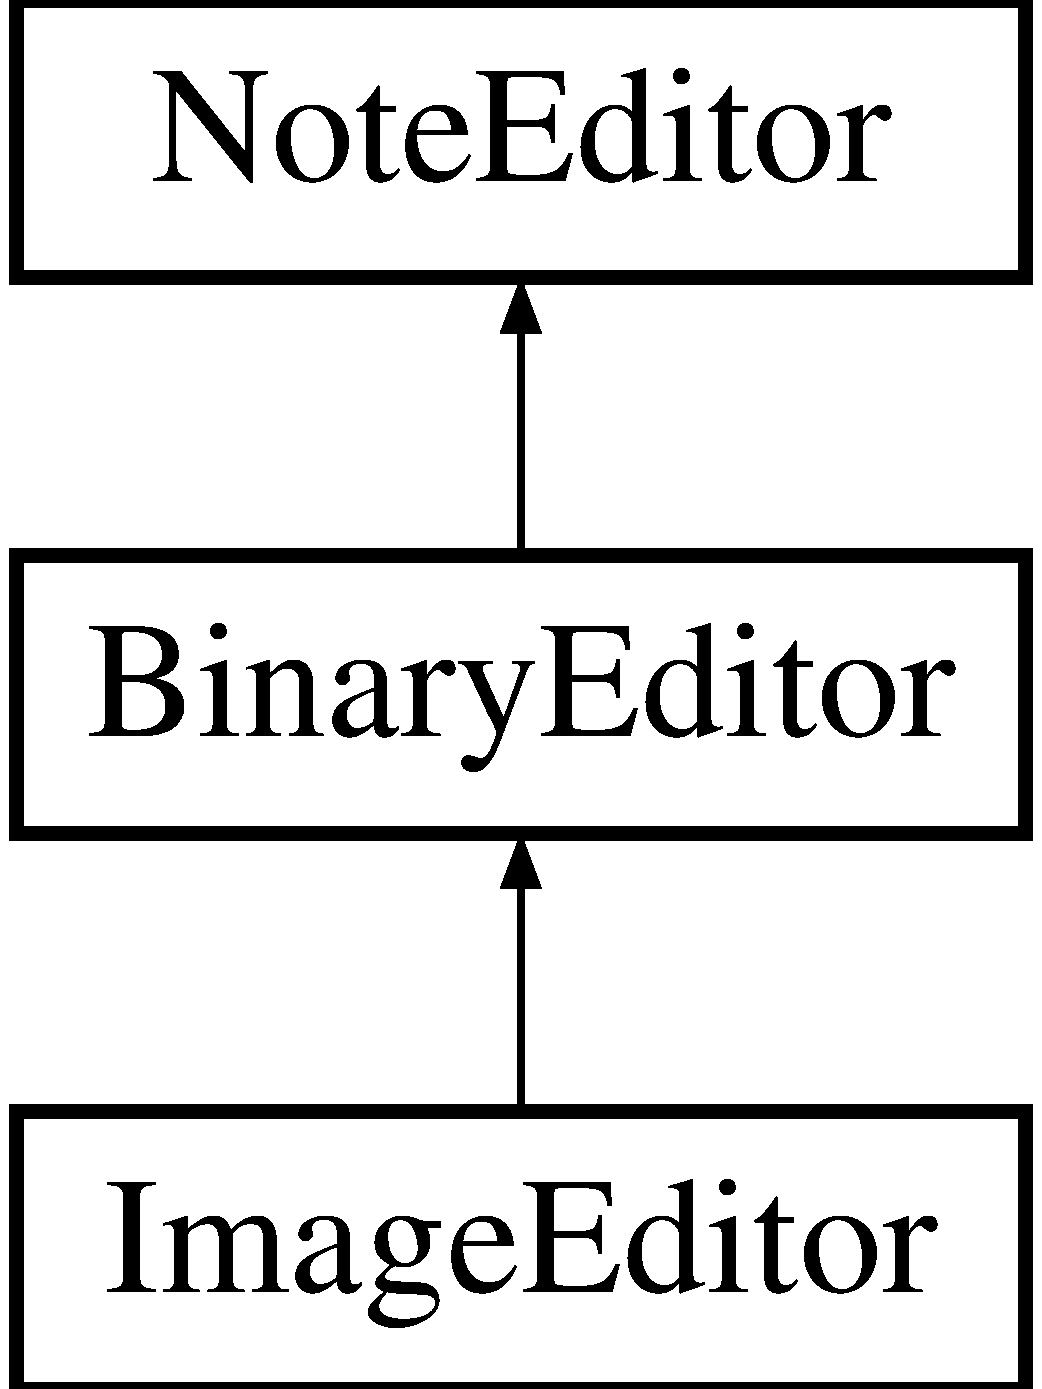
\includegraphics[height=3.000000cm]{classImageEditor}
\end{center}
\end{figure}
\subsection*{\-Public \-Member \-Functions}
\begin{DoxyCompactItemize}
\item 
\hypertarget{classImageEditor_aad6362364edd121eb9078d9bea3afcea}{{\bfseries \-Image\-Editor} (\hyperlink{classImage}{\-Image} $\ast$i, \-Q\-Widget $\ast$parent=0)}\label{classImageEditor_aad6362364edd121eb9078d9bea3afcea}

\item 
\hypertarget{classImageEditor_a8c88f3e1532823b747da313c9c210c2b}{\-Q\-String {\bfseries select\-File} ()}\label{classImageEditor_a8c88f3e1532823b747da313c9c210c2b}

\item 
\hypertarget{classImageEditor_a68ed4fb140109f5d81ce807adef5720e}{void {\bfseries update\-Bin} ()}\label{classImageEditor_a68ed4fb140109f5d81ce807adef5720e}

\end{DoxyCompactItemize}


\-The documentation for this class was generated from the following files\-:\begin{DoxyCompactItemize}
\item 
\-Image.\-h\item 
\-Image.\-cpp\end{DoxyCompactItemize}

\hypertarget{classMainWindow}{\section{\-Main\-Window \-Class \-Reference}
\label{classMainWindow}\index{\-Main\-Window@{\-Main\-Window}}
}
\subsection*{\-Public \-Member \-Functions}
\begin{DoxyCompactItemize}
\item 
\hypertarget{classMainWindow_af9a470d72068ea43f2043b9abbc82bc1}{{\bfseries \-Main\-Window} (\-Q\-Application $\ast$)}\label{classMainWindow_af9a470d72068ea43f2043b9abbc82bc1}

\item 
\hypertarget{classMainWindow_a25bf76ca93b08fc079fd09814152c40c}{void {\bfseries note\-Creator} (\hyperlink{classNote}{\-Note} $\ast$)}\label{classMainWindow_a25bf76ca93b08fc079fd09814152c40c}

\item 
\hypertarget{classMainWindow_a2939ef699376c697046634edaa1307c7}{\hyperlink{classQListEditorItem}{\-Q\-List\-Editor\-Item} $\ast$ {\bfseries new\-Item} (\hyperlink{classNote}{\-Note} $\ast$)}\label{classMainWindow_a2939ef699376c697046634edaa1307c7}

\end{DoxyCompactItemize}


\-The documentation for this class was generated from the following files\-:\begin{DoxyCompactItemize}
\item 
\-Main\-Window.\-h\item 
\-Main\-Window.\-cpp\end{DoxyCompactItemize}

\hypertarget{classNote}{\section{\-Note \-Class \-Reference}
\label{classNote}\index{\-Note@{\-Note}}
}
\-Inheritance diagram for \-Note\-:\begin{figure}[H]
\begin{center}
\leavevmode
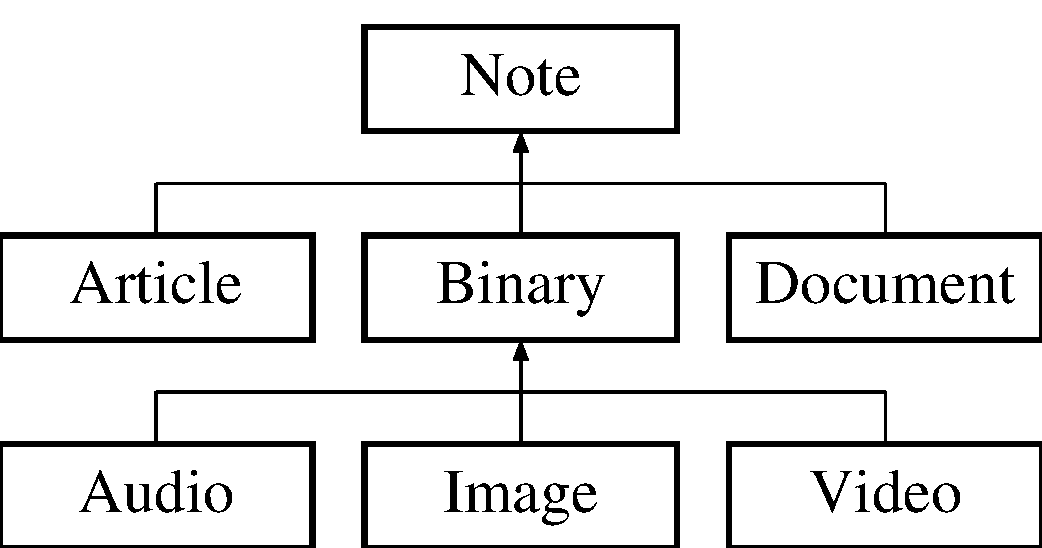
\includegraphics[height=3.000000cm]{classNote}
\end{center}
\end{figure}
\subsection*{\-Public \-Member \-Functions}
\begin{DoxyCompactItemize}
\item 
\hypertarget{classNote_a3138630ccdb6b6d422424fa94b6e4222}{{\bfseries \-Note} (const \-Q\-String \&ty, const \-Q\-String \&i, const \-Q\-String \&tt)}\label{classNote_a3138630ccdb6b6d422424fa94b6e4222}

\item 
\hypertarget{classNote_afac5dd460bebdc9f52f265b0c01f54df}{\-Q\-String \& {\bfseries get\-Id} ()}\label{classNote_afac5dd460bebdc9f52f265b0c01f54df}

\item 
\hypertarget{classNote_ad2630e09ed1356d80f1db4283cd9e4be}{\-Q\-String \& {\bfseries get\-Type} ()}\label{classNote_ad2630e09ed1356d80f1db4283cd9e4be}

\item 
\hypertarget{classNote_aef7f23af8457fede2bc63f91f32d4d0c}{\-Q\-String \& {\bfseries get\-Title} ()}\label{classNote_aef7f23af8457fede2bc63f91f32d4d0c}

\item 
\hypertarget{classNote_a86584195d7aa4a2cc1673447741c98b2}{void {\bfseries set\-Title} (const \-Q\-String \&tt)}\label{classNote_a86584195d7aa4a2cc1673447741c98b2}

\item 
\hypertarget{classNote_a2d7ffa23fe66a9e3749fc172f490350b}{void {\bfseries set\-Modified} (const bool m)}\label{classNote_a2d7ffa23fe66a9e3749fc172f490350b}

\item 
\hypertarget{classNote_abe3ea587b0371292768ce5b6cccfc796}{bool {\bfseries is\-Modified} () const }\label{classNote_abe3ea587b0371292768ce5b6cccfc796}

\item 
\hypertarget{classNote_a277285eef69e663a22180860f6c2f75c}{void {\bfseries set\-Loaded} (const bool l)}\label{classNote_a277285eef69e663a22180860f6c2f75c}

\item 
\hypertarget{classNote_a4bd73aa83650b929464c3f52d6e8e008}{bool {\bfseries get\-Loaded} () const }\label{classNote_a4bd73aa83650b929464c3f52d6e8e008}

\item 
\hypertarget{classNote_ac41c579a824b2343f969f9ab6cc4ad23}{\-Q\-String {\bfseries get\-W\-S} () const }\label{classNote_ac41c579a824b2343f969f9ab6cc4ad23}

\item 
\hypertarget{classNote_a1307f7d1b6bfbfc6d21dca0de8cc9d2e}{void {\bfseries set\-W\-S} (const \-Q\-String \&p=\char`\"{}\char`\"{})}\label{classNote_a1307f7d1b6bfbfc6d21dca0de8cc9d2e}

\item 
\hypertarget{classNote_aba4239202c30b1bf7780168e5785669d}{virtual void {\bfseries add\-Sub\-Note} (\hyperlink{classNote}{\-Note} $\ast$n)}\label{classNote_aba4239202c30b1bf7780168e5785669d}

\item 
\hypertarget{classNote_a8215d0746043be730aa9a38d7d3285f9}{virtual void {\bfseries add\-Sub\-Note} (\hyperlink{classNote}{\-Note} $\ast$n, unsigned int)}\label{classNote_a8215d0746043be730aa9a38d7d3285f9}

\item 
\hypertarget{classNote_a3d294d3e99587a0ad11a3e7c34b5ce5a}{virtual void {\bfseries remove\-Sub\-Note} (unsigned int)}\label{classNote_a3d294d3e99587a0ad11a3e7c34b5ce5a}

\item 
\hypertarget{classNote_ab5e66e683b06741279d1d985415d7aa6}{virtual \hyperlink{classNote}{\-Note} $\ast$ {\bfseries get\-Sub\-Note} (unsigned int pos=0)}\label{classNote_ab5e66e683b06741279d1d985415d7aa6}

\item 
\hypertarget{classNote_a9ac7c1fdeff4f4c5abc16a00d3363e7c}{bool {\bfseries operator==} (const \hyperlink{classNote}{\-Note} $\ast$n) const }\label{classNote_a9ac7c1fdeff4f4c5abc16a00d3363e7c}

\item 
\hypertarget{classNote_ae461ebd3ed6cefc5120467ce9e8a0c54}{bool {\bfseries operator$<$} (const \hyperlink{classNote}{\-Note} $\ast$n) const }\label{classNote_ae461ebd3ed6cefc5120467ce9e8a0c54}

\item 
\hypertarget{classNote_a445fbd0c16993baf1c13c0afed75edb2}{bool {\bfseries less} (const \hyperlink{classNote}{\-Note} $\ast$n) const }\label{classNote_a445fbd0c16993baf1c13c0afed75edb2}

\item 
\hypertarget{classNote_a61c1426d4ebaa250b0f5824686ab0418}{virtual \-Q\-Text\-Stream \& {\bfseries save} (\-Q\-Text\-Stream \&)=0}\label{classNote_a61c1426d4ebaa250b0f5824686ab0418}

\item 
\hypertarget{classNote_a7085a1f824cf244f0ce8b83294bbffc6}{\-Q\-String {\bfseries to\-H\-T\-M\-L} ()}\label{classNote_a7085a1f824cf244f0ce8b83294bbffc6}

\item 
\hypertarget{classNote_a5126f046068ca9d4762685c4f9b1b131}{virtual void {\bfseries makehtmlbody} (\-Q\-Xml\-Stream\-Writer $\ast$qw)=0}\label{classNote_a5126f046068ca9d4762685c4f9b1b131}

\item 
\hypertarget{classNote_ae677cec085c722e939736823d3b6c242}{virtual \-Q\-String {\bfseries to\-T\-E\-X} ()=0}\label{classNote_ae677cec085c722e939736823d3b6c242}

\item 
\hypertarget{classNote_a14650fab181136a122541b83d51b24f5}{virtual \-Q\-String {\bfseries to\-T\-E\-X\-T} ()=0}\label{classNote_a14650fab181136a122541b83d51b24f5}

\item 
\hypertarget{classNote_a2cdb1d951f9983306c3d937c1a4a76ac}{virtual \hyperlink{classNoteEditor}{\-Note\-Editor} $\ast$ {\bfseries get\-Editor} (\-Q\-Widget $\ast$parent=\-N\-U\-L\-L)=0}\label{classNote_a2cdb1d951f9983306c3d937c1a4a76ac}

\end{DoxyCompactItemize}
\subsection*{\-Protected \-Member \-Functions}
\begin{DoxyCompactItemize}
\item 
\hypertarget{classNote_afd8122ada6839ee48f0d92f5646186a0}{virtual void {\bfseries load} ()=0}\label{classNote_afd8122ada6839ee48f0d92f5646186a0}

\item 
\hypertarget{classNote_a3b20f80c2cf8511f0581e28d4927b6ee}{void {\bfseries create\-Tex\-Header} (\-Q\-Buffer $\ast$)}\label{classNote_a3b20f80c2cf8511f0581e28d4927b6ee}

\end{DoxyCompactItemize}
\subsection*{\-Protected \-Attributes}
\begin{DoxyCompactItemize}
\item 
\hypertarget{classNote_a5196ce9d01fe207b10bdc9f8c874053c}{\hyperlink{classNoteEditor}{\-Note\-Editor} $\ast$ {\bfseries editor}}\label{classNote_a5196ce9d01fe207b10bdc9f8c874053c}

\item 
\hypertarget{classNote_a277563af352bd04c5603bdb0bb30869e}{\-Q\-String {\bfseries path\-W\-S}}\label{classNote_a277563af352bd04c5603bdb0bb30869e}

\item 
\hypertarget{classNote_ae8e10911c66931c9285925e1760816fd}{\-Q\-String {\bfseries title}}\label{classNote_ae8e10911c66931c9285925e1760816fd}

\item 
\hypertarget{classNote_a9edcd23344e067ded660deb97bc5ca4a}{bool {\bfseries loaded}}\label{classNote_a9edcd23344e067ded660deb97bc5ca4a}

\item 
\hypertarget{classNote_aaa3ed93cab78b04eebb5b5ba52722871}{bool {\bfseries modified}}\label{classNote_aaa3ed93cab78b04eebb5b5ba52722871}

\item 
\hypertarget{classNote_aeae11c0f8281ba3bfc7ec907cc9cf0b9}{bool {\bfseries deleted}}\label{classNote_aeae11c0f8281ba3bfc7ec907cc9cf0b9}

\item 
\hypertarget{classNote_a76bf0fff374aed4c754c262eeffc62bc}{\-Q\-Byte\-Array $\ast$ {\bfseries file}}\label{classNote_a76bf0fff374aed4c754c262eeffc62bc}

\item 
\hypertarget{classNote_ad1def1d9f3e46da1b0a577ac17c73401}{\-Q\-Buffer $\ast$ {\bfseries buffer}}\label{classNote_ad1def1d9f3e46da1b0a577ac17c73401}

\end{DoxyCompactItemize}


\subsection{\-Detailed \-Description}
\-Correspond au schéma de base pour une \hyperlink{classNote}{\-Note} contenant\-: \-Un titre \-Un workspace \-Un \-I\-D \-Un espace de stockage pour les exports et le prototype de toutes les fonctions obligatoirement nécessaire à une \hyperlink{classNote}{\-Note} un type d'éditeur i.\-e. un graphisme spécifique 

\-The documentation for this class was generated from the following files\-:\begin{DoxyCompactItemize}
\item 
\-Note.\-h\item 
\-Note.\-cpp\end{DoxyCompactItemize}

\hypertarget{classNoteEditor}{\section{\-Note\-Editor \-Class \-Reference}
\label{classNoteEditor}\index{\-Note\-Editor@{\-Note\-Editor}}
}
\-Inheritance diagram for \-Note\-Editor\-:\begin{figure}[H]
\begin{center}
\leavevmode
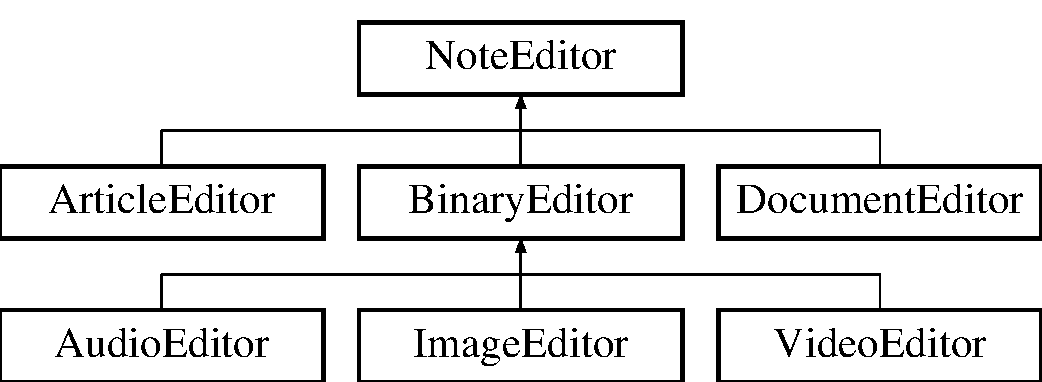
\includegraphics[height=3.000000cm]{classNoteEditor}
\end{center}
\end{figure}
\subsection*{\-Public \-Slots}
\begin{DoxyCompactItemize}
\item 
\hypertarget{classNoteEditor_a1a4c673bba10ffabcc1ee9f51a924ce2}{void {\bfseries tabed} (int)}\label{classNoteEditor_a1a4c673bba10ffabcc1ee9f51a924ce2}

\item 
\hypertarget{classNoteEditor_a273e283bf7ffce87bda4a4dbb6bb6f00}{void {\bfseries title\-Mod} (\-Q\-String)}\label{classNoteEditor_a273e283bf7ffce87bda4a4dbb6bb6f00}

\end{DoxyCompactItemize}
\subsection*{\-Public \-Member \-Functions}
\begin{DoxyCompactItemize}
\item 
\hypertarget{classNoteEditor_a47c957c09b49e3b66d6d022cbc43eb27}{{\bfseries \-Note\-Editor} (\hyperlink{classNote}{\-Note} $\ast$n, \-Q\-Widget $\ast$parent=0)}\label{classNoteEditor_a47c957c09b49e3b66d6d022cbc43eb27}

\item 
\hypertarget{classNoteEditor_abf981dc0ad529ef84aec07b3676456ab}{\hyperlink{classNote}{\-Note} \& {\bfseries get\-Ressource} () const }\label{classNoteEditor_abf981dc0ad529ef84aec07b3676456ab}

\end{DoxyCompactItemize}
\subsection*{\-Public \-Attributes}
\begin{DoxyCompactItemize}
\item 
\hypertarget{classNoteEditor_aec807709a39702dbdf3fac3cc9e16438}{\-Q\-Label $\ast$ {\bfseries html}}\label{classNoteEditor_aec807709a39702dbdf3fac3cc9e16438}

\item 
\hypertarget{classNoteEditor_af85b66c4bec552de741f1e2e95bf07da}{\-Q\-Label $\ast$ {\bfseries tex}}\label{classNoteEditor_af85b66c4bec552de741f1e2e95bf07da}

\item 
\hypertarget{classNoteEditor_acbd842c53fac8acf986ca89e30a29563}{\-Q\-Label $\ast$ {\bfseries text}}\label{classNoteEditor_acbd842c53fac8acf986ca89e30a29563}

\end{DoxyCompactItemize}
\subsection*{\-Protected \-Attributes}
\begin{DoxyCompactItemize}
\item 
\hypertarget{classNoteEditor_a8d452060ccda16b6fa01dd3888cdd26e}{\-Q\-V\-Box\-Layout $\ast$ {\bfseries main\-Lay}}\label{classNoteEditor_a8d452060ccda16b6fa01dd3888cdd26e}

\item 
\hypertarget{classNoteEditor_ae8addf8ac12731112c793d2d6655587b}{\-Q\-Tab\-Widget $\ast$ {\bfseries tabs}}\label{classNoteEditor_ae8addf8ac12731112c793d2d6655587b}

\item 
\hypertarget{classNoteEditor_a15706f3ea231b43f81c94dc264654d73}{\-Q\-Scroll\-Area $\ast$ {\bfseries area}}\label{classNoteEditor_a15706f3ea231b43f81c94dc264654d73}

\item 
\hypertarget{classNoteEditor_a9f20e3eb7fb6fef386804d67689480db}{\-Q\-Widget $\ast$ {\bfseries zone}}\label{classNoteEditor_a9f20e3eb7fb6fef386804d67689480db}

\item 
\hypertarget{classNoteEditor_aa4d46395b4ce04546ea559b9c97c76e9}{\-Q\-V\-Box\-Layout $\ast$ {\bfseries zone\-Layout}}\label{classNoteEditor_aa4d46395b4ce04546ea559b9c97c76e9}

\item 
\hypertarget{classNoteEditor_aa064cabc61e851768c410689bf169f39}{\-Q\-Line\-Edit $\ast$ {\bfseries title}}\label{classNoteEditor_aa064cabc61e851768c410689bf169f39}

\item 
\hypertarget{classNoteEditor_a96f175025780f6b0084f8b9e74cda56a}{\hyperlink{classNote}{\-Note} $\ast$ {\bfseries ressource}}\label{classNoteEditor_a96f175025780f6b0084f8b9e74cda56a}

\end{DoxyCompactItemize}


\-The documentation for this class was generated from the following files\-:\begin{DoxyCompactItemize}
\item 
\-Note.\-h\item 
\-Note.\-cpp\end{DoxyCompactItemize}

\hypertarget{classNotesException}{\section{\-Notes\-Exception \-Class \-Reference}
\label{classNotesException}\index{\-Notes\-Exception@{\-Notes\-Exception}}
}
\subsection*{\-Public \-Member \-Functions}
\begin{DoxyCompactItemize}
\item 
\hypertarget{classNotesException_af10aca61d1cb993b62e868f0fe9bf144}{{\bfseries \-Notes\-Exception} (const \-Q\-String \&message)}\label{classNotesException_af10aca61d1cb993b62e868f0fe9bf144}

\item 
\hypertarget{classNotesException_abe69dc0035ff93205ec8aeb1770ab8c5}{\-Q\-String {\bfseries get\-Info} () const }\label{classNotesException_abe69dc0035ff93205ec8aeb1770ab8c5}

\end{DoxyCompactItemize}


\-The documentation for this class was generated from the following file\-:\begin{DoxyCompactItemize}
\item 
\-Q\-Header.\-h\end{DoxyCompactItemize}

\hypertarget{classNotesManager}{\section{\-Notes\-Manager \-Class \-Reference}
\label{classNotesManager}\index{\-Notes\-Manager@{\-Notes\-Manager}}
}


{\ttfamily \#include $<$\-Notes\-Manager.\-h$>$}

\subsection*{\-Public \-Member \-Functions}
\begin{DoxyCompactItemize}
\item 
\hypertarget{classNotesManager_a73a3d9559f50711098932c8db5ee7def}{const \-Q\-String \& {\bfseries get\-Filename} (\hyperlink{classNote}{\-Note} \&n)}\label{classNotesManager_a73a3d9559f50711098932c8db5ee7def}

\item 
\hypertarget{classNotesManager_a6d33fc29d55fe78e9a11f7549d4cab88}{\hyperlink{classNote}{\-Note} $\ast$ {\bfseries get\-Note} (unsigned int i=0)}\label{classNotesManager_a6d33fc29d55fe78e9a11f7549d4cab88}

\item 
\hypertarget{classNotesManager_a9c401bfe7c91ab37a7c8c4db398e92ff}{\hyperlink{classNote}{\-Note} \& {\bfseries get\-Note} (const \-Q\-String \&id)}\label{classNotesManager_a9c401bfe7c91ab37a7c8c4db398e92ff}

\item 
\hypertarget{classNotesManager_a0c6380a0dccd8f477ad5305d7a798126}{\hyperlink{classNote}{\-Note} \& {\bfseries get\-New\-Note} (const \-Q\-String \&type, const \-Q\-String \&title)}\label{classNotesManager_a0c6380a0dccd8f477ad5305d7a798126}

\item 
\hypertarget{classNotesManager_a73b0f85ed9efe1a4e674066b25d8eca0}{void {\bfseries save\-Note} (\hyperlink{classNote}{\-Note} \&n)}\label{classNotesManager_a73b0f85ed9efe1a4e674066b25d8eca0}

\item 
\hypertarget{classNotesManager_a29d032aae2c5c2a95bbd11c8345f05e5}{void {\bfseries delete\-Note} (\hyperlink{classNote}{\-Note} \&n)}\label{classNotesManager_a29d032aae2c5c2a95bbd11c8345f05e5}

\item 
\hypertarget{classNotesManager_adf555cbe01a64c5a68a2ef9a77f4ae3d}{void {\bfseries set\-Deleted} (\hyperlink{classNote}{\-Note} \&n)}\label{classNotesManager_adf555cbe01a64c5a68a2ef9a77f4ae3d}

\item 
\hypertarget{classNotesManager_aa3cc4234acf0e4055a1159348ac01ae0}{void {\bfseries set\-Undeleted} (\hyperlink{classNote}{\-Note} \&n)}\label{classNotesManager_aa3cc4234acf0e4055a1159348ac01ae0}

\item 
\hypertarget{classNotesManager_a8a2a291206a92186102c0a748b348830}{bool {\bfseries is\-Deleted} (\hyperlink{classNote}{\-Note} \&n)}\label{classNotesManager_a8a2a291206a92186102c0a748b348830}

\item 
\hypertarget{classNotesManager_a49b47e2469bc3f6c34a32d160e69ec1d}{unsigned int {\bfseries get\-Nb\-Notes} ()}\label{classNotesManager_a49b47e2469bc3f6c34a32d160e69ec1d}

\item 
\hypertarget{classNotesManager_add6ea86f4a824189c6d05ceaeb0e66bb}{\-Q\-Icon {\bfseries get\-Note\-Icon} (\hyperlink{classNote}{\-Note} $\ast$n)}\label{classNotesManager_add6ea86f4a824189c6d05ceaeb0e66bb}

\item 
\hypertarget{classNotesManager_a5b04a079b9889741a93d1c34d3cc88ae}{void {\bfseries change\-Workspace} ()}\label{classNotesManager_a5b04a079b9889741a93d1c34d3cc88ae}

\end{DoxyCompactItemize}
\subsection*{\-Static \-Public \-Member \-Functions}
\begin{DoxyCompactItemize}
\item 
\hypertarget{classNotesManager_ad1a91e51ba8506c7ae7cd60d06bd075f}{static \hyperlink{classNotesManager}{\-Notes\-Manager} $\ast$ {\bfseries get\-Instance} ()}\label{classNotesManager_ad1a91e51ba8506c7ae7cd60d06bd075f}

\item 
\hypertarget{classNotesManager_abd12bae3c990a408e9ef55aa0d93b675}{static void {\bfseries liberer\-Instance} ()}\label{classNotesManager_abd12bae3c990a408e9ef55aa0d93b675}

\end{DoxyCompactItemize}
\subsection*{\-Friends}
\begin{DoxyCompactItemize}
\item 
\hypertarget{classNotesManager_a883538034e58fc5c0de7d4e4cab3cef7}{class {\bfseries \-Document}}\label{classNotesManager_a883538034e58fc5c0de7d4e4cab3cef7}

\end{DoxyCompactItemize}


\subsection{\-Detailed \-Description}
classe \-Note\-Manager \-Gère la création des \-Notes,leur destruction et gère leurs accès 

\-The documentation for this class was generated from the following files\-:\begin{DoxyCompactItemize}
\item 
\-Notes\-Manager.\-h\item 
\-Notes\-Manager.\-cpp\end{DoxyCompactItemize}

\hypertarget{classQListEditor}{\section{\-Q\-List\-Editor \-Class \-Reference}
\label{classQListEditor}\index{\-Q\-List\-Editor@{\-Q\-List\-Editor}}
}
\subsection*{\-Public \-Slots}
\begin{DoxyCompactItemize}
\item 
\hypertarget{classQListEditor_a7646e05181a114dd6e209c398e924fb6}{void {\bfseries it\-Act\-Clicked} (\-Q\-List\-Widget\-Item $\ast$it)}\label{classQListEditor_a7646e05181a114dd6e209c398e924fb6}

\item 
\hypertarget{classQListEditor_aaa67233bcc7e247efe7da4374eb72151}{void {\bfseries it\-Act\-Double\-Clicked} (\-Q\-List\-Widget\-Item $\ast$it)}\label{classQListEditor_aaa67233bcc7e247efe7da4374eb72151}

\end{DoxyCompactItemize}
\subsection*{\-Signals}
\begin{DoxyCompactItemize}
\item 
\hypertarget{classQListEditor_a0a6f9fbf755ad20aed536e448378ed29}{void {\bfseries it\-Act\-Clicked\-S} (\hyperlink{classQListEditorItem}{\-Q\-List\-Editor\-Item} $\ast$)}\label{classQListEditor_a0a6f9fbf755ad20aed536e448378ed29}

\item 
\hypertarget{classQListEditor_ae1faecd09505cd0ccdce71fe9becbc63}{void {\bfseries it\-Act\-Double\-Clicked\-S} (\hyperlink{classQListEditorItem}{\-Q\-List\-Editor\-Item} $\ast$)}\label{classQListEditor_ae1faecd09505cd0ccdce71fe9becbc63}

\end{DoxyCompactItemize}
\subsection*{\-Public \-Member \-Functions}
\begin{DoxyCompactItemize}
\item 
\hypertarget{classQListEditor_a7d73a55ee3860fef1009ec597934519b}{{\bfseries \-Q\-List\-Editor} (\-Q\-Widget $\ast$parent=\-N\-U\-L\-L)}\label{classQListEditor_a7d73a55ee3860fef1009ec597934519b}

\item 
\hypertarget{classQListEditor_a216f4434999f65861f8bb95253a50861}{void {\bfseries add\-Item} (\hyperlink{classQListEditorItem}{\-Q\-List\-Editor\-Item} $\ast$it\-Act)}\label{classQListEditor_a216f4434999f65861f8bb95253a50861}

\item 
\hypertarget{classQListEditor_ad663e237f1c80b2598c383b771c94d7b}{\hyperlink{classQListEditorItem}{\-Q\-List\-Editor\-Item} $\ast$ {\bfseries take\-Item} (int pos)}\label{classQListEditor_ad663e237f1c80b2598c383b771c94d7b}

\item 
\hypertarget{classQListEditor_ab40df10831d16fb647f5c82b1a25df9c}{void {\bfseries set\-Current\-Item} (\hyperlink{classQListEditorItem}{\-Q\-List\-Editor\-Item} $\ast$item)}\label{classQListEditor_ab40df10831d16fb647f5c82b1a25df9c}

\item 
\hypertarget{classQListEditor_a4ba7ba186b229adc87b9419e06866e05}{void {\bfseries clear} ()}\label{classQListEditor_a4ba7ba186b229adc87b9419e06866e05}

\item 
\hypertarget{classQListEditor_a29e1f37d1577756aa334c3c40f0225c3}{\hyperlink{classQListEditorItem}{\-Q\-List\-Editor\-Item} $\ast$ {\bfseries item} (int pos)}\label{classQListEditor_a29e1f37d1577756aa334c3c40f0225c3}

\end{DoxyCompactItemize}


\-The documentation for this class was generated from the following file\-:\begin{DoxyCompactItemize}
\item 
\-Main\-Window.\-h\end{DoxyCompactItemize}

\hypertarget{classQListEditorItem}{\section{\-Q\-List\-Editor\-Item \-Class \-Reference}
\label{classQListEditorItem}\index{\-Q\-List\-Editor\-Item@{\-Q\-List\-Editor\-Item}}
}


{\ttfamily \#include $<$\-Main\-Window.\-h$>$}

\subsection*{\-Public \-Member \-Functions}
\begin{DoxyCompactItemize}
\item 
\hypertarget{classQListEditorItem_a31857393514604258864a0d60ef0a72f}{{\bfseries \-Q\-List\-Editor\-Item} (const \-Q\-String \&tt, \hyperlink{classNoteEditor}{\-Note\-Editor} $\ast$res, \-Q\-Object $\ast$parent=\-N\-U\-L\-L)}\label{classQListEditorItem_a31857393514604258864a0d60ef0a72f}

\item 
\hypertarget{classQListEditorItem_a04cef2cfa7e131d3c0162716a71a0671}{{\bfseries \-Q\-List\-Editor\-Item} (const \-Q\-Icon \&ico, \hyperlink{classNoteEditor}{\-Note\-Editor} $\ast$res, \-Q\-Object $\ast$parent=\-N\-U\-L\-L)}\label{classQListEditorItem_a04cef2cfa7e131d3c0162716a71a0671}

\item 
\hypertarget{classQListEditorItem_a6609f35d04481c8355f8469182ac0e01}{{\bfseries \-Q\-List\-Editor\-Item} (const \-Q\-Icon \&ico, const \-Q\-String \&tt, \hyperlink{classNoteEditor}{\-Note\-Editor} $\ast$res, \-Q\-Object $\ast$parent=\-N\-U\-L\-L)}\label{classQListEditorItem_a6609f35d04481c8355f8469182ac0e01}

\item 
\hypertarget{classQListEditorItem_af2de55af804abb9966ed3fe769fa822c}{\hyperlink{classNoteEditor}{\-Note\-Editor} $\ast$ {\bfseries get\-Ressource} () const }\label{classQListEditorItem_af2de55af804abb9966ed3fe769fa822c}

\end{DoxyCompactItemize}


\subsection{\-Detailed \-Description}
classe \hyperlink{classMainWindow}{\-Main\-Window} \-Gère la création de l'interface \-Graphique, les liens entre les différents menus ou widgets et les fonctions relatives. 

\-The documentation for this class was generated from the following file\-:\begin{DoxyCompactItemize}
\item 
\-Main\-Window.\-h\end{DoxyCompactItemize}

\hypertarget{classTag}{\section{\-Tag \-Class \-Reference}
\label{classTag}\index{\-Tag@{\-Tag}}
}
\subsection*{\-Public \-Member \-Functions}
\begin{DoxyCompactItemize}
\item 
\hypertarget{classTag_a4b8d9b57f817525b336be7f57c7d4cd0}{{\bfseries \-Tag} (\-Q\-String \&nid, \-Q\-Set$<$ \-Q\-String $>$ t=\-Q\-Set$<$ \-Q\-String $>$())}\label{classTag_a4b8d9b57f817525b336be7f57c7d4cd0}

\item 
\hypertarget{classTag_a1b690fb5385690f454c0283e76818f50}{\-Q\-Set$<$ \-Q\-String $>$ \& {\bfseries get\-Tags\-List} ()}\label{classTag_a1b690fb5385690f454c0283e76818f50}

\item 
\hypertarget{classTag_ad58a79c30b6f7be52bf92f380bf6e5ae}{\-Q\-String \& {\bfseries get\-Noteid} ()}\label{classTag_ad58a79c30b6f7be52bf92f380bf6e5ae}

\item 
\hypertarget{classTag_ac614cfc590e974d1c0fcfe4c80726beb}{void {\bfseries add\-Tags} (\-Q\-Set$<$ \-Q\-String $>$ tags)}\label{classTag_ac614cfc590e974d1c0fcfe4c80726beb}

\item 
\hypertarget{classTag_ab76b419440563072c75085788b45b508}{bool {\bfseries operator==} (\hyperlink{classTag}{\-Tag} \&t)}\label{classTag_ab76b419440563072c75085788b45b508}

\end{DoxyCompactItemize}


\-The documentation for this class was generated from the following files\-:\begin{DoxyCompactItemize}
\item 
tagmanager.\-h\item 
tagmanager.\-cpp\end{DoxyCompactItemize}

\hypertarget{classTagManager}{\section{\-Tag\-Manager \-Class \-Reference}
\label{classTagManager}\index{\-Tag\-Manager@{\-Tag\-Manager}}
}


{\ttfamily \#include $<$tagmanager.\-h$>$}

\subsection*{\-Public \-Member \-Functions}
\begin{DoxyCompactItemize}
\item 
\hypertarget{classTagManager_a7fa940878e143a82e68659126b2f6192}{void {\bfseries liberer\-Instance} ()}\label{classTagManager_a7fa940878e143a82e68659126b2f6192}

\item 
\hypertarget{classTagManager_a8848ee002c31d81493822b2103ab6f87}{\-Q\-List$<$ \hyperlink{classNote}{\-Note} $\ast$ $>$ {\bfseries note\-List\-From\-Tag\-Restriction} (\-Q\-List$<$ \-Q\-String $>$)}\label{classTagManager_a8848ee002c31d81493822b2103ab6f87}

\item 
\hypertarget{classTagManager_ae54ef7fd6982b88a22a77905dac30402}{void {\bfseries updatedictionary} (\-Q\-List$<$ \-Q\-String $>$ tags)}\label{classTagManager_ae54ef7fd6982b88a22a77905dac30402}

\item 
\hypertarget{classTagManager_a691e9e29b5ea11aaca6f2dfe32054503}{\-Q\-Set$<$ \-Q\-String $>$ \& {\bfseries get\-Dictionary} (\-Q\-Set$<$ \-Q\-String $>$ \&s)}\label{classTagManager_a691e9e29b5ea11aaca6f2dfe32054503}

\item 
\hypertarget{classTagManager_a3e7f7e2e04ad5400e51794ebadd09ae7}{void {\bfseries add\-Note\-And\-Tags} (\hyperlink{classNote}{\-Note} \&, \-Q\-Set$<$ \-Q\-String $>$ s)}\label{classTagManager_a3e7f7e2e04ad5400e51794ebadd09ae7}

\item 
\hypertarget{classTagManager_ac3f165f78bd418d8dd33868a6f362a62}{void {\bfseries add\-Tags\-To\-Note} (\-Q\-String \&nid, \-Q\-Set$<$ \-Q\-String $>$ s=\-Q\-Set$<$ \-Q\-String $>$())}\label{classTagManager_ac3f165f78bd418d8dd33868a6f362a62}

\item 
\hypertarget{classTagManager_a8b27158d4d629b4497495bc7491ad2f3}{\-Q\-List$<$ \-Q\-String $>$ \& {\bfseries get\-Tagslist\-For\-Note} (\-Q\-String \&nid)}\label{classTagManager_a8b27158d4d629b4497495bc7491ad2f3}

\end{DoxyCompactItemize}
\subsection*{\-Static \-Public \-Member \-Functions}
\begin{DoxyCompactItemize}
\item 
\hypertarget{classTagManager_af7de9966f3731509eef656f015df32c8}{static \hyperlink{classTagManager}{\-Tag\-Manager} $\ast$ {\bfseries get\-Instance} ()}\label{classTagManager_af7de9966f3731509eef656f015df32c8}

\end{DoxyCompactItemize}


\subsection{\-Detailed \-Description}
\-Correspond au \-Mécanisme de gestion des \-Tags gère\-: \-La correspondance \-Note-\/$>$tags l'ajout/suppresion de\-Tags la récupération des tags de l'extérieur la gestion du dictionnaire de tous les \-Tags 

\-The documentation for this class was generated from the following files\-:\begin{DoxyCompactItemize}
\item 
tagmanager.\-h\item 
tagmanager.\-cpp\end{DoxyCompactItemize}

\hypertarget{classVideo}{\section{\-Video \-Class \-Reference}
\label{classVideo}\index{\-Video@{\-Video}}
}


{\ttfamily \#include $<$\-Video.\-h$>$}

\-Inheritance diagram for \-Video\-:\begin{figure}[H]
\begin{center}
\leavevmode
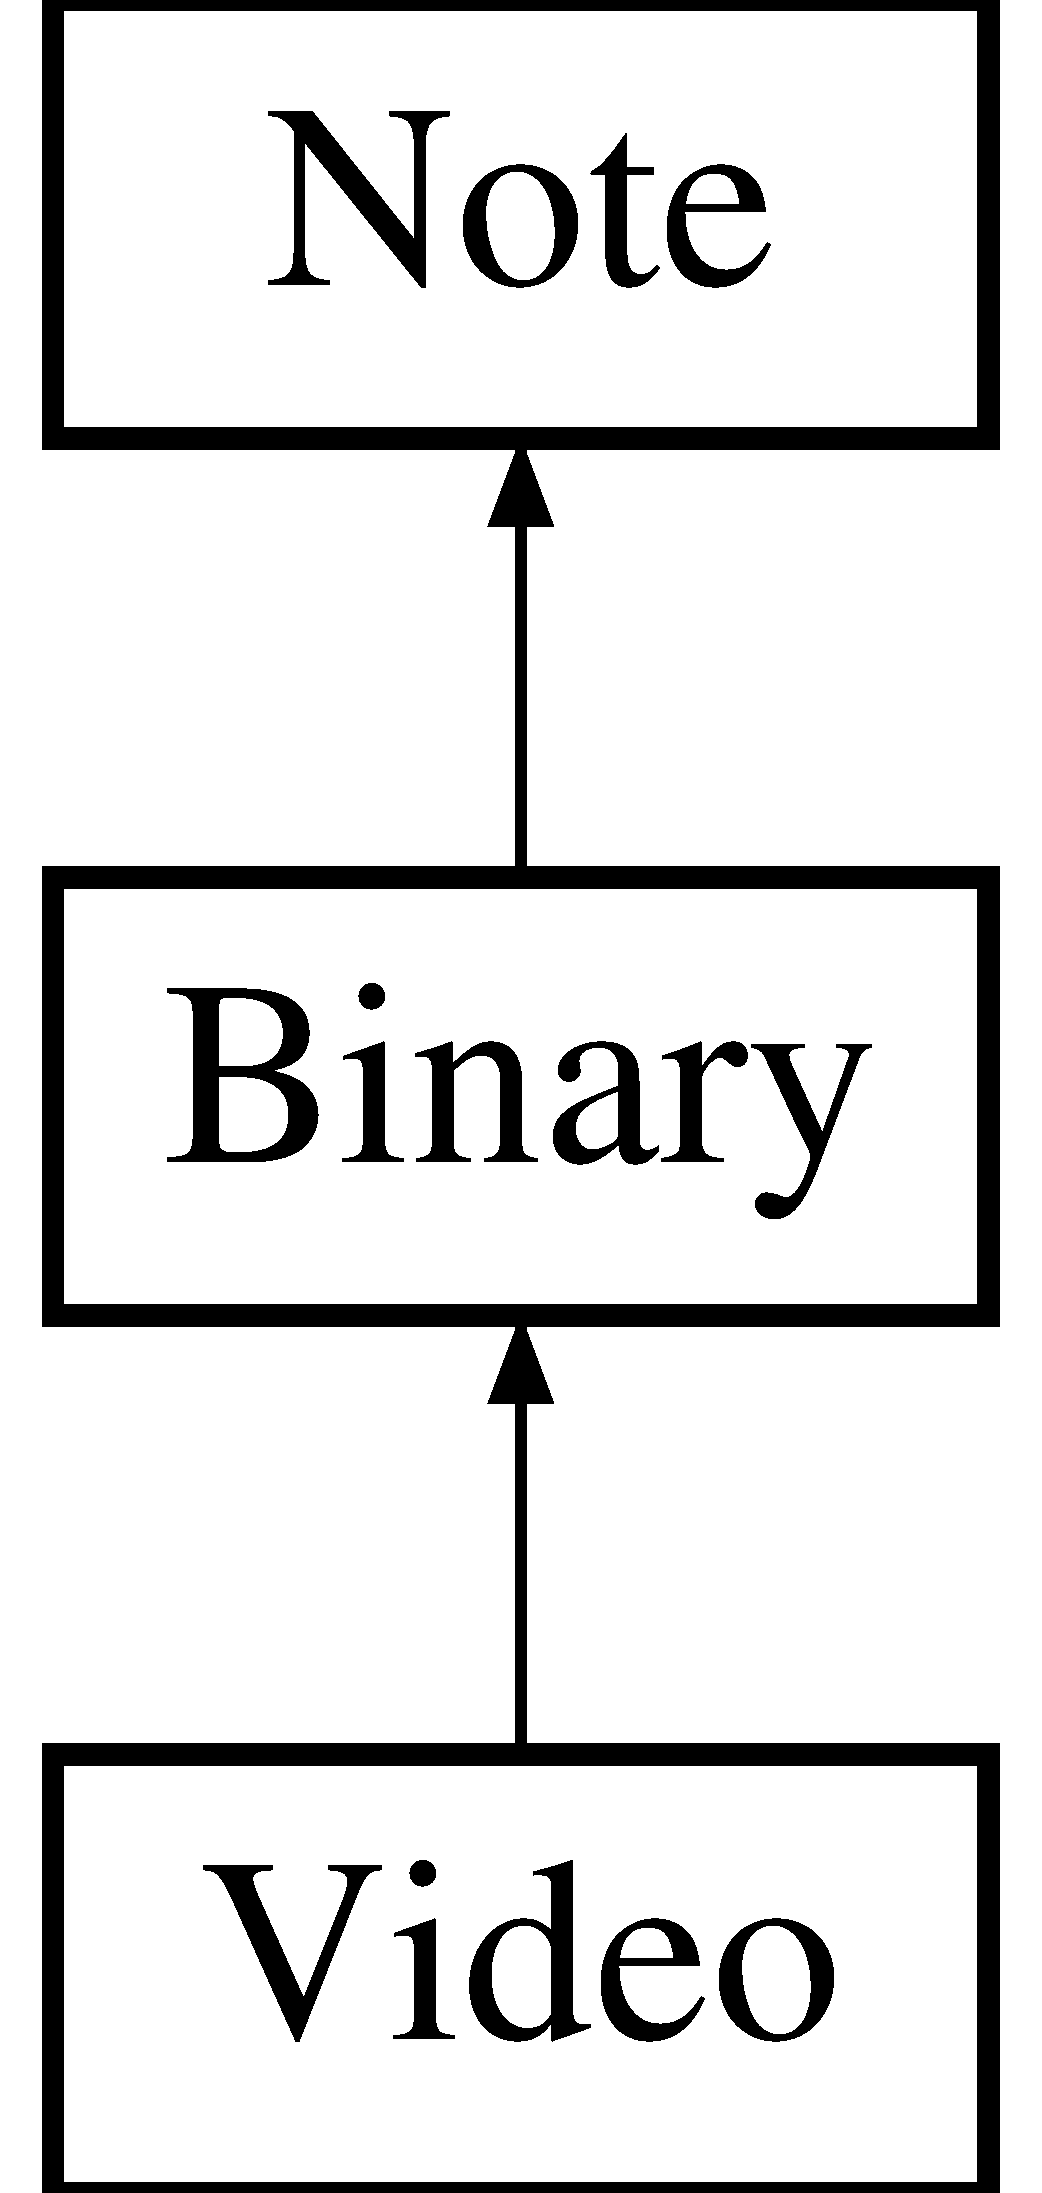
\includegraphics[height=3.000000cm]{classVideo}
\end{center}
\end{figure}
\subsection*{\-Public \-Member \-Functions}
\begin{DoxyCompactItemize}
\item 
\hypertarget{classVideo_a3168a14f309b49637eedc71e34977bae}{{\bfseries \-Video} (const \-Q\-String \&id, const \-Q\-String \&title, const \-Q\-String \&desc=\char`\"{}\char`\"{}, const \-Q\-String \&path=\char`\"{}\char`\"{})}\label{classVideo_a3168a14f309b49637eedc71e34977bae}

\item 
\hypertarget{classVideo_a15663427ca1d41338c05273757556b05}{\-Q\-Text\-Stream \& {\bfseries save} (\-Q\-Text\-Stream \&f)}\label{classVideo_a15663427ca1d41338c05273757556b05}

\item 
\hypertarget{classVideo_a04ebb4918373da74bc061823b26d1ef5}{\hyperlink{classNoteEditor}{\-Note\-Editor} $\ast$ {\bfseries get\-Editor} (\-Q\-Widget $\ast$parent=\-N\-U\-L\-L)}\label{classVideo_a04ebb4918373da74bc061823b26d1ef5}

\item 
\hypertarget{classVideo_a78404c789304e0049fc2f2748c521269}{void {\bfseries makehtmlbody} (\-Q\-Xml\-Stream\-Writer $\ast$qw)}\label{classVideo_a78404c789304e0049fc2f2748c521269}

\item 
\hypertarget{classVideo_a932c6b7632624a17ce95f8d537c6065e}{\-Q\-String {\bfseries to\-T\-E\-X} ()}\label{classVideo_a932c6b7632624a17ce95f8d537c6065e}

\item 
\hypertarget{classVideo_afb84bc4f21ccb46db6e539f5530009de}{\-Q\-String {\bfseries to\-T\-E\-X\-T} ()}\label{classVideo_afb84bc4f21ccb46db6e539f5530009de}

\end{DoxyCompactItemize}


\subsection{\-Detailed \-Description}
\-Correspond à la spécification de \hyperlink{classBinary}{\-Binary} pour contenir\-: une \hyperlink{classVideo}{\-Video} un type d'éditeur i.\-e. un graphisme spécifique et des exports \-H\-T\-M\-L,\-Tex,\-T\-E\-X\-T correspondants 

\-The documentation for this class was generated from the following files\-:\begin{DoxyCompactItemize}
\item 
\-Video.\-h\item 
\-Video.\-cpp\end{DoxyCompactItemize}

\hypertarget{classVideoEditor}{\section{\-Video\-Editor \-Class \-Reference}
\label{classVideoEditor}\index{\-Video\-Editor@{\-Video\-Editor}}
}
\-Inheritance diagram for \-Video\-Editor\-:\begin{figure}[H]
\begin{center}
\leavevmode
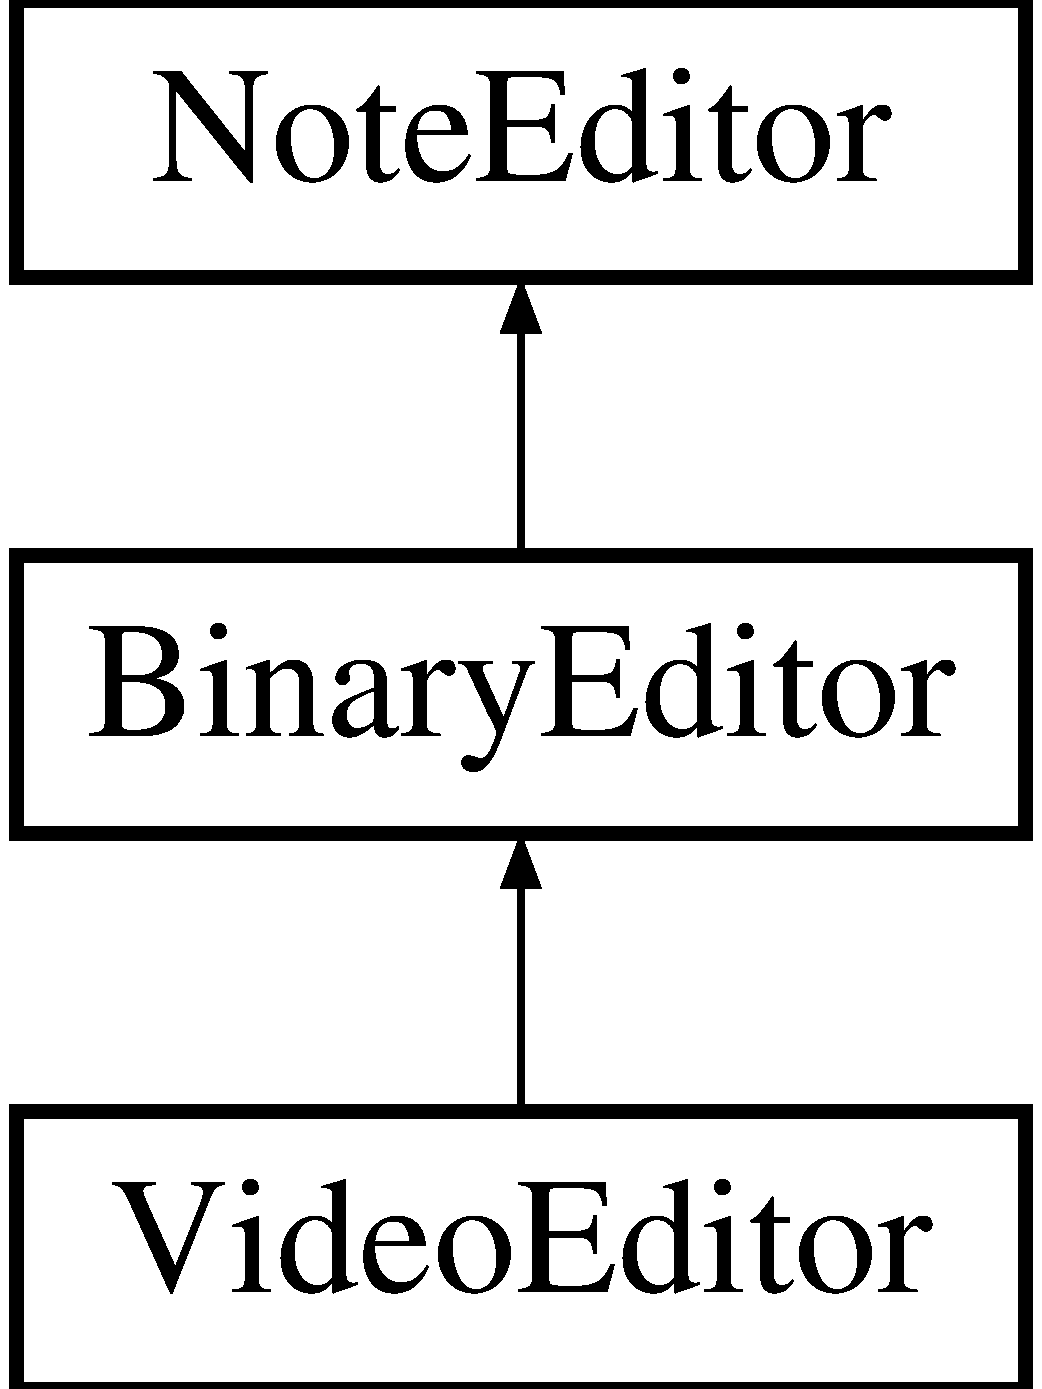
\includegraphics[height=3.000000cm]{classVideoEditor}
\end{center}
\end{figure}
\subsection*{\-Public \-Member \-Functions}
\begin{DoxyCompactItemize}
\item 
\hypertarget{classVideoEditor_a05925389f4dd395bbd43605481326018}{{\bfseries \-Video\-Editor} (\hyperlink{classVideo}{\-Video} $\ast$v, \-Q\-Widget $\ast$parent=0)}\label{classVideoEditor_a05925389f4dd395bbd43605481326018}

\item 
\hypertarget{classVideoEditor_a856f5c81afa9fb9e339ca67414c8a8aa}{\-Q\-String {\bfseries select\-File} ()}\label{classVideoEditor_a856f5c81afa9fb9e339ca67414c8a8aa}

\item 
\hypertarget{classVideoEditor_a01cad2eadd5d701c248d5b390cd5318a}{void {\bfseries update\-Bin} ()}\label{classVideoEditor_a01cad2eadd5d701c248d5b390cd5318a}

\end{DoxyCompactItemize}


\-The documentation for this class was generated from the following files\-:\begin{DoxyCompactItemize}
\item 
\-Video.\-h\item 
\-Video.\-cpp\end{DoxyCompactItemize}

\hypertarget{classWorkspace}{\section{\-Workspace \-Class \-Reference}
\label{classWorkspace}\index{\-Workspace@{\-Workspace}}
}


{\ttfamily \#include $<$\-Workspace.\-h$>$}

\subsection*{\-Public \-Member \-Functions}
\begin{DoxyCompactItemize}
\item 
\hypertarget{classWorkspace_af16c8a4fe636d1cc98ac2eddfdfc2859}{{\bfseries \-Workspace} (const \-Q\-String \&p=\char`\"{}.\char`\"{})}\label{classWorkspace_af16c8a4fe636d1cc98ac2eddfdfc2859}

\item 
\hypertarget{classWorkspace_a86c8e878fb7982d984ad7a432a54dc29}{\-Q\-String {\bfseries get\-Path} ()}\label{classWorkspace_a86c8e878fb7982d984ad7a432a54dc29}

\item 
\hypertarget{classWorkspace_a3aec5fd32dcdbb1102dd5fdd68314310}{void {\bfseries set\-Path} (const \-Q\-String \&p=\char`\"{}.\char`\"{})}\label{classWorkspace_a3aec5fd32dcdbb1102dd5fdd68314310}

\item 
\hypertarget{classWorkspace_aa5d1d2a63c5c29d387f47c0d93483afd}{\-Q\-List$<$ \-Q\-String $>$ {\bfseries list\-Notes} ()}\label{classWorkspace_aa5d1d2a63c5c29d387f47c0d93483afd}

\item 
\hypertarget{classWorkspace_ad91083cb3da49ca2049bf15122db4dcc}{\-Q\-List$<$ \-Q\-String $>$ {\bfseries list\-Notes\-D} ()}\label{classWorkspace_ad91083cb3da49ca2049bf15122db4dcc}

\item 
\hypertarget{classWorkspace_aacd690ce475b83a0d01c7234a66a4762}{\-Q\-List$<$ \-Q\-String $>$ {\bfseries list\-Tags} ()}\label{classWorkspace_aacd690ce475b83a0d01c7234a66a4762}

\item 
\hypertarget{classWorkspace_a72442ff60a4b1a26a0974c8de9e4b81d}{void {\bfseries note\-To\-D} (const \-Q\-String \&path)}\label{classWorkspace_a72442ff60a4b1a26a0974c8de9e4b81d}

\item 
\hypertarget{classWorkspace_af33b62cf9249df5e5aed7ae2ed92b3d0}{void {\bfseries deleted\-To\-N} (const \-Q\-String \&path)}\label{classWorkspace_af33b62cf9249df5e5aed7ae2ed92b3d0}

\item 
\hypertarget{classWorkspace_ab6c5f71ce638d24afb51a2b649efbaa5}{\-Q\-String {\bfseries get\-Type} (const \-Q\-String \&path)}\label{classWorkspace_ab6c5f71ce638d24afb51a2b649efbaa5}

\item 
\hypertarget{classWorkspace_a85737d20bd3fc7dfa8fa67cd061e25ca}{\-Q\-String {\bfseries get\-Tags} (const \-Q\-String \&path)}\label{classWorkspace_a85737d20bd3fc7dfa8fa67cd061e25ca}

\item 
\hypertarget{classWorkspace_aa210a7b48674979f52c01a914204bde4}{bool {\bfseries is\-Note} (const \-Q\-String \&path)}\label{classWorkspace_aa210a7b48674979f52c01a914204bde4}

\item 
\hypertarget{classWorkspace_a52703ebffe544e4c68489ed5d902d79c}{void {\bfseries add\-Note} (const \-Q\-String \&path, const \-Q\-String \&type, const \-Q\-List$<$ \-Q\-String $>$ \&tags)}\label{classWorkspace_a52703ebffe544e4c68489ed5d902d79c}

\item 
\hypertarget{classWorkspace_ae63099b7935de34ecde80bb20a38d6d1}{void {\bfseries update\-Note} (const \-Q\-String \&path, const \-Q\-String \&type, const \-Q\-List$<$ \-Q\-String $>$ \&tags)}\label{classWorkspace_ae63099b7935de34ecde80bb20a38d6d1}

\item 
\hypertarget{classWorkspace_a83d87b636daffae2f8e91b3837ab450a}{void {\bfseries delete\-Note} (const \-Q\-String \&path)}\label{classWorkspace_a83d87b636daffae2f8e91b3837ab450a}

\item 
\hypertarget{classWorkspace_ac87ace25faf72934d2febf64defec99e}{void {\bfseries check} ()}\label{classWorkspace_ac87ace25faf72934d2febf64defec99e}

\end{DoxyCompactItemize}


\subsection{\-Detailed \-Description}
\-Gère la création physique des notes, les dossiers de travail gère la sauvegarde des notes leurs suppression/restauration 

\-The documentation for this class was generated from the following files\-:\begin{DoxyCompactItemize}
\item 
\-Workspace.\-h\item 
\-Workspace.\-cpp\end{DoxyCompactItemize}

\printindex
\end{document}
